\documentclass[a4paper,10pt]{article}

%\usepackage[utf8]{inputenc}
\usepackage{graphicx}
\usepackage{url}
\usepackage{float}
\usepackage{times}
\usepackage{multirow}
\usepackage{listings}
\usepackage{times}
\usepackage{paralist}
\usepackage{epsfig}
\usepackage{subfigure}
\usepackage[hypertex]{hyperref}
\usepackage{subfigure}
\usepackage{color}
\usepackage{ifpdf}
\usepackage{wrapfig}

\usepackage{texdraw}
\usepackage{epsf}
\usepackage{array}
\usepackage{cite}
\usepackage{enumitem}
\usepackage{verbatim}
\usepackage{setspace}
\sloppy
\usepackage{geometry}



\newcommand{\I}[1]{\textit{#1}}
\newcommand{\B}[1]{\textbf{#1}}
\newcommand{\BI}[1]{\textbf{\textit{#1}}}
\newcommand{\T}[1]{\texttt{#1}}
\newcommand{\dctf}{dC$_{25}$ }
\newcommand{\dctfnsp}{dC$_{25}$}
\newcommand{\atf}{A$_{25}$ }
\newcommand{\dco}{dC$_{1}$ }
\newcommand{\atfnsp}{A$_{25}$}
\newcommand{\dconsp}{dC$_{1}$}
\newcommand{\aonsp}{A$_{1}$}
\newcommand{\ao}{A$_{1}$ }
\newcommand{\ato}{A$_{1}$ }
\newcommand{\ahl}{$\alpha$HL }
\newcommand{\ahlnsp}{$\alpha$HL}
\newcommand{\prim}{$^{\prime}$ }
\newcommand{\primnsp}{$^{\prime}$}


\pdfpagewidth 8.5in
\pdfpageheight 11in 

\setlength\topmargin{0in}
\setlength\headheight{0in}
\setlength\headsep{0in}
\setlength\textheight{9in}
\setlength\textwidth{6.5in}
\setlength\oddsidemargin{0in}
\setlength\evensidemargin{0in}
\setlength\parindent{0.1in}
\setlength\parskip{0.25em}

\ifpdf
 \DeclareGraphicsExtensions{.pdf, .jpg, .png}
\else
 \DeclareGraphicsExtensions{.eps, .ps}
\fi

\newcommand{\jha}[1]{ {\textcolor{red} { ***Jha: #1 }}}

\begin{document}
\title{\LARGE % Investigating Scale-Out Performance of 
% Loosely-Coupled Simulations Using Multiple Distributed Resources on the TeraGrid.
  Scale-Up and Scale-Out of Ensemble-based Simulations}

% \author{Principal Investigator: Shantenu Jha$^{1,2}$ \\
% Co-Principal Investigator: Joohyun Kim$^{1}$ \\ 
% Co-Principal Investigator: Yaakoub El Khamra$^{3}$\\\
%    \small{\emph{$^{1}$Center for Computation \& Technology, Louisiana State University, Baton Rouge, 
% USA}}
% \\
%   \small{\emph{$^{2}$Department of Computer Science, Louisiana State
%       University, Baton Rouge, USA}}
% \\
%   \small{\emph{$^{3}$Texas Advanced Computing Center TACC, University of Texas, Austin, USA}}}

\newif\ifdraft
%\drafttrue
\ifdraft
\newcommand{\amnote}[1]{ {\textcolor{magenta} { ***AM: #1c }}}
\newcommand{\jhanote}[1]{ {\textcolor{red} { ***SJ: #1 }}}
\newcommand{\michaelnote}[1]{ {\textcolor{blue} { ***MM: #1 }}}
\newcommand{\yyenote}[1]{ {\textcolor{green} { ***YYE: #1 }}}
\else
\newcommand{\amnote}[1]{}
\newcommand{\jhanote}[1]{}
\newcommand{\michaelnote}[1]{ {\textcolor{blue} { ***MM: #1 }}}
\newcommand{\yyenote}[1]{ {}}
\fi

%\date{15 July 2010}

\date{}

\maketitle

\subsection*{Summary:} 

This work is built on the extensive efforts over the past several years that have carried out with a wide range of computational science and computer science projects. In this TRAC request, we propose to use TeraGrid resources to investigate a broad-range of science and computer science problems using loosely-coupled ensemble-based simulations.  We will use multiple TeraGrid resources both in concurrent usage mode, as well as individual resources to study several scientific problems. We are developing  cyberinfrastructure that will enable the collective utilization of TeraGrid resources.  Specifically, in this proposal we request XXXXM SUs for five distinct projects: (1) understanding translocation of nucleic acid in $\alpha$-Hemolysin protein pores; (2) elucidating the underlying mechanism of metabolite binding assisted folding of SAM-I riboswitches and other riboswitches, (3) atomistic simulations of physiological systems, (4) atomistic simulations of bi-layered composites, and, (5) developing and enhancing the understanding of distributed applications and testing the  scale-out performance of a range of applications.  Project 3 will be carried out as part of a collaboration with Prof. Peter Coveney (UCL, Yale); Projects 3 and 5c are part of an international collaboration between TeraGrid and DEISA that is being led the PI and co-PI Prof. Coveney (involving
funding from both the NSF and the EU). The projects for which resources are being requested are all funded projects -- mostly at the National/International level, and some by local resources.  Additionally, the request for XXXXM SUs in this proposal is based upon the projected science problems as outlined below as well as a proven track {\it record of successfully} utilising more than YYYYM SUs in the recent past.

\section{Results From Prior Awards}


\jhanote{This should list out (i) prior awards and what they were for, (ii) scientific progress and understanding that arose and (ii) publications as a result of prior awards.}

\jhanote{Yaakoub/Joohyun: Our award/project number for last years TRAC is MCB090174.
  Please mention resource usage statistics, be sure to mention that we've used 100\% well before
  the expiry. Mention allocation swapping between machines}

\jhanote{Publications arising from clast TRAC: (i) Project 1: JCTC and a publication on ABF are in the works; (ii) Riboswtich -- in addition to NAR, we have ECMLS and others (Joohyun to fix), (iii) UCL is listed in prior.tex so ok, (iv) Project 4, TeraGrid-talk, DEISA Interop talk, and publication in process, but also reference Cybertools publications -- ccgrid and others}


This group has multiple publications arising from earlier TRAC Awards. Initial results from Project 1 supported by the most recent TRAC award to PI Jha (MCB090174) was selected as the cover article of a leading scientific journal~\cite{jctc_cover}.  \begin{wrapfigure}{r}{0.28\textwidth}
 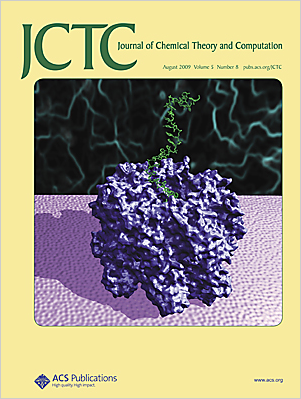
\includegraphics[width=0.28\textwidth]{jctc_cover2.png}
 \caption{\footnotesize JCTC Cover Article}
 \label{cover}
\end{wrapfigure}
Using the previous TRAC allocations, we have performed all-atom MD simulations for the SAM-I riboswtich study.  We have reported our scientific results in recent conferences~\cite{ecmls10}, as well a recently published journal article in the prestigious Nucleic Acids Research\cite{SAM-I-NAR2009} (Impact Factor $>$ 7.0). On the basis of these publications, we have enhanced our scope by expanding our interests \& simulations to other riboswitches, such as TPP riboswitches and recurrent RNA structural motifs such as K-turn, towards a comprehensive understanding of the mechanisms of SAM riboswitches.  Also, we added the complementary computational approaches such as RNA secondary structure prediction in addition to all-atom MD simulations, and our initial effort was presented in the workshop, "Emerging Computational Methods for the Life Sciences" in ACM HPDC 2010\cite{ecmls10}. 

Previously we have used TeraGrid resources to conduct a binding affinity study of the protease inhibitor saquinavir with G48V and L90M containing mutatants which showed good agreement with experiment \cite{Stoica2008}. % uring SuperComputing 2007 we used
Using Lonestar (TG allocation number TG-ASC070019T) to expand this work by running 10ns-long simulations on 5 different HIV protease systems bound to 5 different FDA-approved drugs: amprenavir, indinavir, lopinavir, ritonavir, and saquinavir. We compared our binding energy results for each of the 5 protease genotypes in the MDR set to experimental values published in \cite{Ohtaka2003}. Our results showed varying correlations to experimental trends, with the 5 ritonavir systems showing good correlation to experimental whilst the 5 saquinavir systems showed poor correlation. In light of these results further work was done both on Lonestar (TG allocation numbers TG-ASC070019T and TG-DMR070014N) and more recently Ranger (TG allocation numbers A-rfUser1 and TG-ASC090009) to determine whether repeating the study as an ensemble of MD models would improve correlations. The results showed significantly improved correlations and have led us to refine our simulation protocol and reparameterise a number of inhibitors. An article focussed primarily on our work on the lopinavir bound system has recently been accepted for publication \cite{Sadiq2010}.

In addition to this we have performed a study into the comparative dynamics of different liganded forms of reverse transcriptase, concluding that the binding of the inhibitors efavirenz and nevirapine alter the motions of the catalytically important fingers domain of RT and that these motions are uncorrelated to fluctuations in the drug binding energy (as yet unpublished). We also performed preliminary investigations into the efficacy of the ensemble methodology for calculating binding affinities on NVP bound systems, again concluding that the convergence properties are improved over single trajectory. These results also allowed us to differentiate binding affinity of the L100I and L100I/K103N sequences from the wildtype using simulations of the ligand bound enzyme alone which indicates that they do not significantly affect the creation of the binding pocket. All this work was performed using Ranger. 

These simulations were orchestrated using our automated simulation tool, the Binding Affinity Calculator (BAC), which makes use of AHE \cite{coveney2007,zasada2009} to deploy and run simulations and then retrieve data. Two papers describing this tool and its potential use as a clinical support tool have been published\cite{Sadiq2008, Sadiq2008a}. The BAC allows us to distribute the simulation and analysis sections of our workflow over a number of geographically disparate locations. The mutation and hydration of crystal structure based models takes place on local resources at UCL, using the AMBER software suite, while the actual simulations can be performed in NAMD either on TeraGrid or UKNational Grid Service (NGS) computers and/or EU DEISA grid. The final analysis of the resultant trajectories, either on local recources or the NGS, is performed using the AMBER MD suite of codes. In the last year, BAC has been extended to allow the simulation of the epidermal growth factor receptor (EGFR) and the molecular dynamics code GROMACS \cite{Hess2008}. This new functionality has facilitated a study of the binding of three inhibitors (AEE788, AFN941 and getfitinib) bound to EGFR, performed on Ranger.

In the area of bio-minerals our previous simulations have utilized periodic boundaries on the clay sheets, allowing a simulation cell to represent an infinite clay platelet \cite{JPCC_2007,Thyveetil,Thyveetil_JACS, Soft_Matter1}. These large-scale, fully atomistic simulations, approached the size of a physically realistic platelet. From this, we were able to calculate mesoscopic and macroscopic properties directly from molecular dynamics simulations in the absence of finite-size effects of both clay nanocomposites\cite{JPCC_2007,Thyveetil, Soft_Matter1} and bio-composites~\cite{Thyveetil_JACS}.  Using resources from TG-ASC070019T we extended these simulations to calculate the mechanical response of poly(ethylene oxide) polymer-clay nanocomposites, separating the response into contributions from the polymer and clay mineral layer~\cite{Soft_Matter1}. This separation technique allowed us to determine how the clay-polymer elastic properties change with distance from the clay surface. This is the first time the effect of mineral layers on the elastic modulus of polymeric materials in the vicinity of a mineral surface has been calculated. This result is a vital first step to understanding the enhancement mechanism of nanocomposites and the role of the very large surface area of the clay mineral layer on the surrounding medium.  We have also examined the mechanisms by which clay mineral layers buckle in clay-polymer nanocomposites under compressive stress. We find that a clay sheet remains stable in a flat state until a critical compressive strain is reached, at which point it buckles, and regains its uncompressed area. Over this buckling transition, the Poisson ratio of the clay sheets turns negative, a property which has been predicted for 2-dimensional sheets ~\cite{Soft_Matter2}. This is the first time such behaviour has been seen in a molecular simulation of mineral layers. The large scale allowing us to probe large buckling wavelengths that are inhibited in smaller scale simulation.
% To simulate a realistically sized clay platelet required very large scale simulations, made possible using the resources available via the LRAC allocation.

We have also used previous TRAC allocation for CO$_2$ sequestration studies and reservoir characterization studies. These studies were composed of running an ensemble of independent simulations followed by an anaylsis step, and iterating until a termination criteria is met.  Since the simulations are indpendent, they can be distributed across TeraGrid resources, with a sufficiently abstract and sophisticated workflow manager.  We have begun developing an rudimentary distributed autonomic framework -- Lazarus ~\cite{gmac}, using which we are able to select multiple TeraGrid machines concurrently, dynamically optimize the work-load and gain deep insights. This is a natural continuation of our award winning work in 2008 (TeraGrid 2008 Performance Challenge Award)~\footnote{\url{http://www.cct.lsu.edu/~sjha/select_publications/tg08-performance-award.pdf}}. Beside the obvious science results ~\cite{TG10yye00}, we learned a great deal about scale-out behavior and management of ensembles of large scale simulations, the need for fault tolerance and autonomic behavior, as well as the promising possibilities of combining Grid and Cloud environments. This work has resulted in several publications \cite{Cloud1,Cloud2,MSEScience,TG10yye00} and presentations as well as a Masters degree~\cite{Elkhamra2009}.


\section{Scientific Projects}

A common underlying theme of all the scientific projects proposed here, are that they are composed of simulations that involve multiple (loosely-coupled, or uncoupled) ensembles; thus these applications are ideal candidates for the collective usage of the multiple TeraGrid resources for faster time-to-solutions. However, for a myriad set of complex reasons (including misguided NSF oversight of the TeraGrid~\cite{dpa-grid2009} application-level capabilities and software environment.), it remains difficult to utilize multiple computational TeraGrid resources concurrently towards the solution of a single problem instance.  Not only will this proposal further the science that can arise by using multiple concurrent resources, this proposal will also further and harden the ability to use multiple resources and make it available to the broader TG user community, i.e., although the focus is domain-specific computational science this project will also address the challenges in effective usage of distributed resources.

The five scientific projects we propose to investigate in this proposal, are all currently funded by a range of Federal, local and International Funding Agencies.  We are actively pursuing several opportunities to continue the scientific (See \S Supporting Grants); results from previous TRAC awards form the basis of multiple proposals that are currently under review (totalling \$4M);

\section*{Project 1: Nucleic Acid Translocation through Alpha-Hemolysin Nanopore}

The translocation of polynucleotides across membranes is a fundamental biological process, with important technological and medical relevance.  The translocation process is complex and is influenced by a range of factors including the diameter and inner surface of the pore, the secondary structure of the polymer, and interactions between polymer and protein. We have performed non-equilibrium constant velocity-steered molecular dynamics (cv-SMD) simulations of nucleic acid molecule translocation through the protein nanopore $\alpha$-hemolysin (\ref{fig:edge}) and used Jarzynski's identity% ~\cite{jarz} 
to determine the associated free energy profiles. Constant velocity-steered molecular dynamics~\cite{namd} (cv-SMD) is a type of non-equilibrium simulation that connects an atom or center of mass of a group of atoms via a harmonic spring moved at constant velocity. Cv-SMD has the advantage of a well defined wall-clock and simulated time-frame for a given translocation distance, allowing the induction of high-speed translocation in a consistent manner.

\begin{figure}[!h]
  \begin{center}
    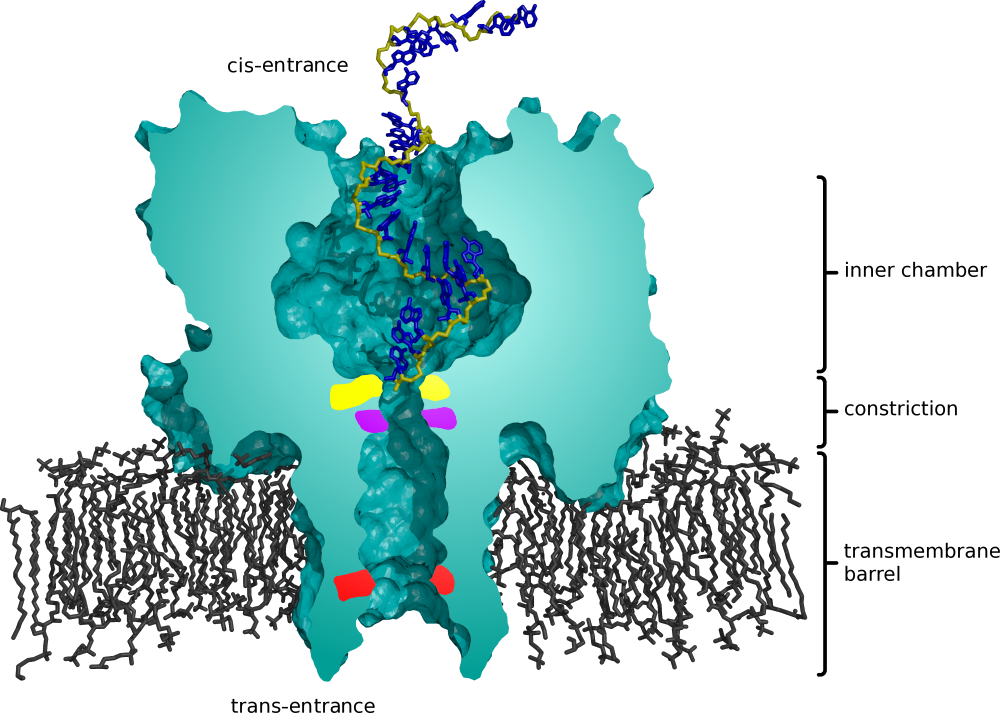
\includegraphics[width=5.0in]{ahl_labelled13}
  \end{center}
  \caption{\small Figure representing the starting configuration of a 3\prim
    led \atf translocation simulation~\cite{jctc_cover}. The
    heptameric protein pore \ahl (green) is inserted into a lipid
    bilayer (black). Features of the translocating molecule include
    the backbone of \atf (dark yellow) and the nucleic acid bases
    (blue). The $trans$-entrance is at the bottom of the pore; taking
    the $trans$-entrance of \ahl as a reference point at 0~{\AA},
    other notable features include protein residue Leu-135 at 13~{\AA}
    (red), Met-113 at 43~{\AA} (pink), Lys-147 at 45~{\AA} (light
    yellow), and the $cis$-entrance at the top of the protein at
    95~{\AA}. The $cis$-entrance is 28~{\AA} in diameter, the wide
    section of the pore running from the $cis$-entrance to residue
    Lys-147 is termed the inner chamber and is up to 46~{\AA}
    wide. The constriction marked by residues Lys-147 and Met-113 is
    14~{\AA} wide, while the transmembrane barrel runs from the
    constriction to the $trans$-entrance and is around 20~{\AA} wide;
    the $trans$-entrance is 24~{\AA} wide. The C3\prim carbon atom of
    the 3\prim end residue of \atf is aligned with the center of mass
    of the C$_{\alpha}$ atoms of protein residue 111, which lies at
    the mouth of the constriction, just above residue Lys-147. For the
    sake of clarity, water molecules, sodium and chloride ions are not
    displayed (they are found along the entire length of the pore).}
  \label{fig:edge}
\end{figure} 


With this approach we have been able to explain the observed differences in experimental translocation time through the nanopore between polyadenosine and polydeoxycytidine. Poly(A) and poly(dC) molecules of 100-200 bases in length exhibit a 20-fold difference in translocation time through \ahl in SCCR experiments~\cite{akeson}. The translocation of both 25 base polynucleotides and single nucleotides through $\alpha$-hemolysin has been investigated. An example of our results that qualitatively agree with experimental findings can be seen in Fig.~\ref{full_trans_local}. These simulations are computationally intensive as they employ models with atomistic level resolution; in addition to their size, these systems are challenging to study due to the time-scales of translocation of large asymmetric molecules. Our simulations have provided insight into the role of the interactions between the nucleic acid molecules and the protein-pore. Mutated protein-pores have provided confirmation of residue-specific interactions between nucleotides and the protein-pore. By harnessing such molecular dynamics simulations, we have gained new physical insight into the translocation process.

This work has been published in the {\em Journal of Chemical Theory and Computation}~\cite{jctc_cover}, where we pushed cv-SMD to new limits, testing the validity of the method for a larger translocating molecule and higher atom count system than previously attempted at such relatively low pulling speeds. We showed that an interaction between a positively charged lysine residue of the pore interior and the negatively charged nucleotide phosphate groups give rise to peaks in the free energy profiles. We also highlighted key ion interactions that play a role in these phosphate-lysine interactions, pointing to important considerations for future computational scientists to consider. The work that has been published so far covers relatively low sampled instances of nucleotide and single nucleotide translocation through wild type and mutated protein pores, yielding good results and has established the groundwork for further publications.

 \begin{figure}[!h]
  \begin{center}
\subfigure{\label{fig:fulltrans-a}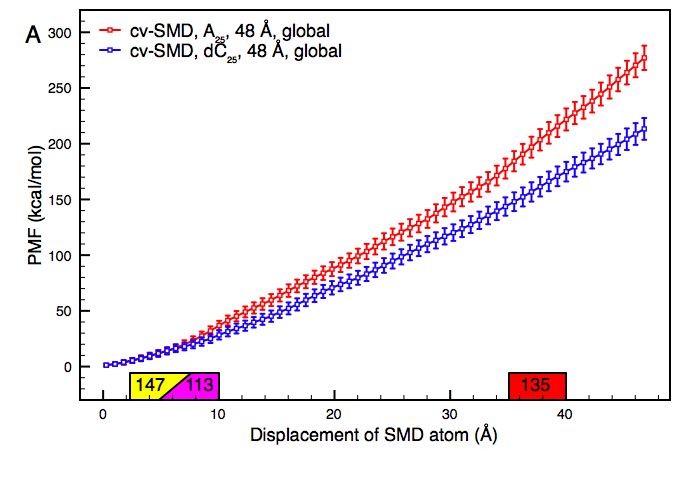
\includegraphics[scale=0.33]{full_trans_16sample_cv-SMD_A25_vs_dC25_nice_adjusted}}
\subfigure{\label{fig:fulltrans-b}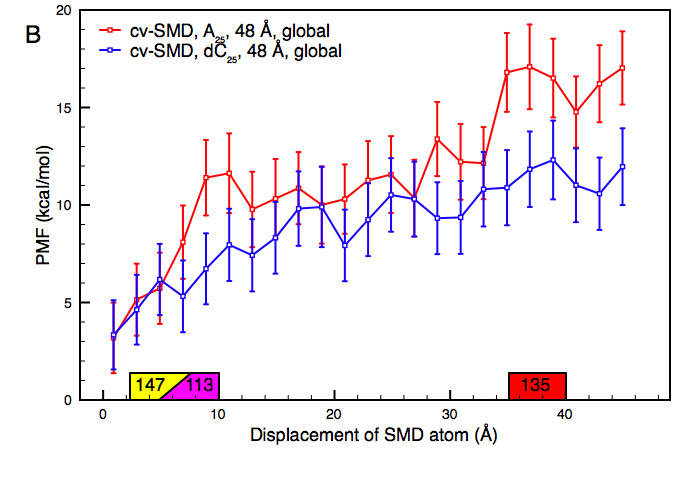
\includegraphics[scale=0.33]{full_trans_16sample_cv-SMD_A25_vs_dC25_local_nice_adjusted}}  
    \end{center}
   \caption[Local and global free energy profiles of \atf and \dctf translocation from the top of the constriction to the bottom of the $trans$-entrance of wild type \ahl]{\small Local and global free energy profiles of \atf and \dctf translocation from the top of the constriction to the bottom of the $trans$-entrance of wild type \ahlnsp. A) Global free energy profile of \atf and \dctf
translocation; each profile was derived from 16 samples, calculated using a bin width of 0.75~{\AA}. Labelled along the $x$-axis are protein residues Met-147, Lys-113, and Leu-135. The residue labels span 5~{\AA} from when the pulled atom to first
phosphate atom passes the labelled residue. The free energy estimate for \atf is $\sim$30\% higher than that of \dctf at the end of the 48~{\AA} reaction coordinate. The plots show discrimination of \atf and \dctf beyond the error bars after 11~{\AA} of translocation. The gradients of both profiles gradually increase, which is in line with expectations that pulling additional nucleotides into the confining dimensions of the transmembrane barrel raises the energetic barriers to further translocation. B) Local free energy profiles of \atf and \dctf translocation; each profile was derived from 16 samples, calculated using a bin width of 2~{\AA}. For these systems, the local environments lead to consistently higher energetic barriers to translocation for \atfnsp. The \atf profiles also exhibits larger peaks than \dctfnsp, most notably at 9~{\AA} and 37~{\AA}.}
  \label{full_trans_local}
\end{figure}

Using the TRAC grant that was awarded to us last year, we have significantly improved the sampling of these results, and amassed further data. For the latest set of data, each profile is calculated from 16 samples (instead of 2-4 samples previously), which has greatly improved the quality and reliability of the data. Systems \dctfnsp-WT,  \dconsp-WT, \atfnsp-WT,  \aonsp-WT,  and \dctfnsp-Mut (see Table~\ref{table:systems1}), were included in the JCTC publication with a low number of samples; these now stand at 16 samples each. Systems \dconsp-Mut, \atfnsp-Mut, and \aonsp-Mut, were not previously explored and now have full 16 sample data-sets. Using these data-sets we have been able to make conclusions such as the negligible impact of the nucleotide base sterics, and are able to point to nucleotide base stacking as  one of the causes for the experimentally observed difference between poly(A) and poly(dC) translocation times.

Additionally, over the last year we have used the molecular models established in the cv-SMD simulations to test the system using an alternative translocation method. The method we examined was Adaptive Biasing Force (ABF). Here the translocating atom (and thus the attached molecule) is moved with a biasing force, which acts to overcome energy barriers in order to translocate along a reaction coordinate. The biasing force adapts to the free energy landscape on-the-fly, calculating the free energy and biasing force based on the forces acting on the atom in question, and applying the force directly to that atom. In this way, ABF surpasses the need for certain approximations to be made related to the use of Jarzynski's Equality and the requirement of a stiff cv-SMD harmonic spring, allowing us to assess the impact that these approximations had on the cv-SMD data. Furthermore, ABF does not constrain the biased atom in axes orthogonal to the reaction coordinate, allowing enhanced sampling of the reaction coordinate. So far, we have examined key ABF simulation parameters to allow for the exploration of the \ahl-nucleotide systems, and have produced single sample free energy profiles for \atfnsp-ABF and \dctfnsp-ABF (see Table~\ref{table:systems1}). This work is now being prepared for submission to the Journal of Computational Science (Expected September 2010).

\begin{table}[!h]
\begin{center}
  \caption{The translocation molecules and pore types to be simulated. `Wild Type' indicates \ahl with no mutated residues; `Mutant' indicates \ahl mutant L147M.\newline }
\label{table:systems1}
\begin{tabular}{| c | c | c | c | c | c |}
\hline
Pulling & System & \ahl Type & Nucleotide & Nucleotides & Samples \\
Method & Name &  & Base &  & Performed \\
\hline
cv-SMD & \aonsp-WT & Wild Type & Adenine & 1 & 16/16  \\
cv-SMD & \atfnsp-WT & Wild Type & Adenine & 25 & 16/16  \\
cv-SMD & \dconsp-WT & Wild Type & Deoxycytosine & 1 & 16/16  \\
cv-SMD & \dctfnsp-WT & Wild Type & Deoxycytosine & 25 & 16/16 \\
cv-SMD & \aonsp-Mut & Mutant & Adenine & 1 & 16/16  \\
cv-SMD & \atfnsp-Mut & Mutant & Adenine & 25 & 16/16  \\
cv-SMD & \dconsp-Mut & Mutant & Deoxycytosine & 1 & 16/16  \\
cv-SMD & \dctfnsp-Mut & Mutant & Deoxycytosine & 25 & 16/16  \\
ABF & \atfnsp-ABF & Wild Type & Adenine & 25 & 1  \\
ABF & \dctfnsp-ABF & Wild Type & Deoxycytosine & 25 & 1  \\
\hline
\end{tabular}
\end{center}
\end{table}

We have ascertained that to allow for the production of quality data that may be compared to our cv-SMD results, we require multi-sample (at least 4) data-sets of systems  \atfnsp-ABF-$\zeta$5k, \dctfnsp-ABF-$\zeta$5k,  \aonsp-ABF-$\zeta$5k,  and \dconsp-ABF-$\zeta$5k (see Table~\ref{table:systems2}). For these simulations, there is a key ABF parameter, $\zeta$, that dictates how many timesteps the biased atom is required to exist within the boundaries of a particular bin along the reaction coordinate before the biasing force in applied. This parameter influences the impact of non-equilibrium effects, the average speed of translocation, plus the computational cost, and its optimum value is highly sensitive to the size and flexibility of the translocating molecule. Therefore, we will also be performing simulations where the $\zeta$ value is pushed to more computationally intensive limits to determine its full impact on the data quality. These systems are \atfnsp-ABF-$\zeta$20k, \dctfnsp-ABF-$\zeta$20k,  \atfnsp-ABF-$\zeta$80k, \dctfnsp-ABF-$\zeta$80k, as listed in Table~\ref{table:systems2}.


\begin{table}[!h]
\begin{center}
  \caption{The translocation molecules and pore types to be simulated. `Wild Type' indicates \ahl with no mutated residues; `Mutant' indicates \ahl mutant L147M.\newline }
\label{table:systems2}
\begin{tabular}{| c | c | c | c | c | c | c |}
\hline
Pulling & System & \ahl Type & Nucleotide & Nucleotides & Samples & CPU Hours \\
Method & Name &  & Base &  & Performed & Required\\
\hline
ABF & \atfnsp-ABF-$\zeta$5k & Wild Type & Adenine & 25 & 4 & 39,732 \\
ABF & \atfnsp-ABF-$\zeta$20k & Wild Type & Adenine & 25 & 4 & 158,928 \\
ABF & \atfnsp-ABF-$\zeta$80k & Wild Type & Adenine & 25 & 2  & 317,856 \\
ABF & \dctfnsp-ABF-$\zeta$5k & Wild Type & Deoxycytosine & 25 & 4 & 39,732 \\
ABF & \dctfnsp-ABF-$\zeta$20k & Wild Type & Deoxycytosine & 25 & 4 & 158,928  \\
ABF & \dctfnsp-ABF-$\zeta$80k & Wild Type & Deoxycytosine & 25 & 2 & 317,856 \\
ABF & \aonsp-ABF-$\zeta$5k & Wild Type & Adenine & 1 & 4 &  39,732 \\
ABF & \dconsp-ABF-$\zeta$5k & Wild Type & Deoxycytosine & 1 & 4 & 39,732 \\
\hline
\end{tabular}
\end{center}
\end{table}

For systems of this size (approximately 325,000 atoms) and for the timescales of interest, it is necessary to use a HPC parallel MD Engine.  The project uses the parallel MD code NAMD and as also led to a grid-enabled version of NAMD developed by us to perform steered MD simulations including the capability to connect to distributed haptic devices (c.f. SC05 HPC Analytics Award). This work is currently funded by the UK's EPSRC (equivalent to the US NSF).  We use NAMD on 512 processors typically. We have used Ranger, Kraken and QueenBee extensively for earlier simulations for this project. The CPU hour requirements for these simulations are listed in Table~\ref{table:systems2}. For ABF simulations using a 325,000 atom model, 2~ns of simulation typically takes about 9.7 hours on Kraken. To complete an ABF sample, we estimate that the following number of nanoseconds are required - 4ns, 16ns, and 64ns for $\zeta$=5k, $\zeta$=20k, and $\zeta$=80k respectively. Therefore a single sample $\zeta$=5k simulations will require 9,933 CPU hours, and a 4 sample free energy profile will hence require 39,732 CPU hours. A single sample $\zeta$=20k simulations will require 39,732 CPU hours, and a 4 sample free energy profile will hence require 158,928 CPU hours. A single sample $\zeta$=80k simulations will require 158,928 CPU hours, and a 2 sample free energy profile will hence require 317,856 CPU hours. The total requirement for the remainder of this project is therefore 1,112,496 CPU hours. About 1.2M SUs more are required to finish sampling these remaining systems.  Therefore we ask for 1.2M to be allocated to us for use on this project. To be used primarily on Kraken.

\section*{Project 2: Computational Study of non-coding Functional RNAs: Folding Dynamics and Binding mechanism of Riboswitches}

Continuing our efforts toward a comprehensive understanding of molecular mechanisms of Riboswitch RNAs that displays a remarkable example of non-coding RNA gene regulatory systems, we plan to carry out and advance our research of the Riboswitch RNAs with computational approaches in the cycle of this allocation period.  Our research goals during coming years can be understood readily with the pipeline illustrated in Fig.~\ref{fig:ribo-pipeline}. 

With the proposed pipeline, we aim the holistic approach to investigate folding dynamics of ribsowtich RNAs and closely related RNA-ligand binding affinity.  This is somewhat contrast to our strategy of the previous years during which we have exclusively employed all-atom Molecular Dynamics simulations.  Indeed, combining multiple computational approaches that differ in their physical principles increase a chance to achieve comprehensive understanding of the complex biological process carried out by riboswitch RNAs.  The entire pipeline comprises three steps; the first step represents the Boltzmann Ensemble (BE) sampling of RNA secondary structures, the second step is about the 3D modeling from 2D structure information, and the third step carries out the conformational sampling.  Note that the sampling with the first step is executed with RNA secondary structure prediction algorithms, employing the nearest-neighbor energy model and thermodynamics parameters experimentally estimated.  The third step is carried out with all-atom MD simulations.  Between them, the second step represents the 3-D molecular modeling from the 2-D information.  WIth the requested allocation, we mainly carry out computation corresponding to the first and the third.  The BE sampling for the first step is conducted with SFold package\cite{ding2006}.  This type of sampling is typically carried out without parallel implementation, but recently, with the development of a novel runtime environment, we demonstrated the parallel sampling of RNA secondary structures using scalable HPC resources in the paper presented in "Emerging Computational Methodologies in Life Science"~\cite{ecmls10}. For all-atom MD simulations, protocols similar to previous years will be used as described below.  Also, we plan to implement massively parallel secondary structure sampling using GPU-accelarated implementation.   As a matter of fact, our pipeline represents the energy landscape perspective that interprets the folding dynamics of a RNA with statistical treatment of an ensemble of structures distributed in the pertinent energy landscape~\cite{onuchic1997}, which has been successfully applied for protein folding but not fully applied for RNA folding\cite{cupal1997}. In our pipeline,  the entire folding configuration space is efficiently explored by RNA secondary structure sampling and successively atomistic MD simulations explore the relevant basins of attraction starting from the configurations sampled.     

Importantly, note that while our pipeline can serve as a de-novo tool for RNA structure prediction from a sequence when used together, our pipeline also can be used as a tool box that is able to carry out different physics-based calculations corresponding to each layer, i.e., RNA secondary structure prediction, 3D modeling, and all atom MD simulations for different scientific aims.  This is particularly related to the fact that the nature of RNA folding occurs through the hierarchical manner, implying that the first and the third steps can deal with its own biophysical problems but later findings can be combined for the holistic understanding.  Furthermore, we emphasize that considering the use of various computational approaches whose performance relies upon the availability of effective parallel implementation, our research benefits only from Teragrid like federated, distributed and massively parallel resources.

\begin{figure}
\begin{center}
  \subfigure[]{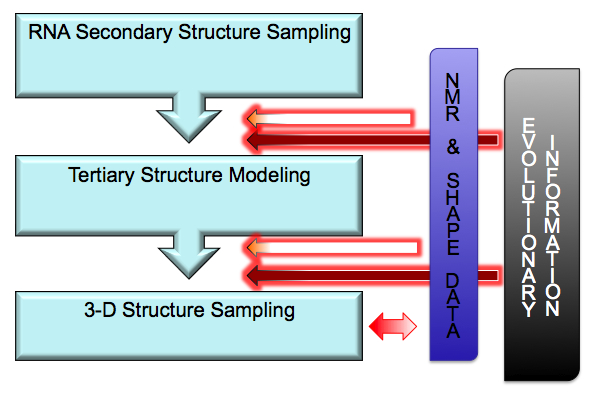
\includegraphics[scale=0.33]{flowchart-pipeline}}
  \subfigure[]{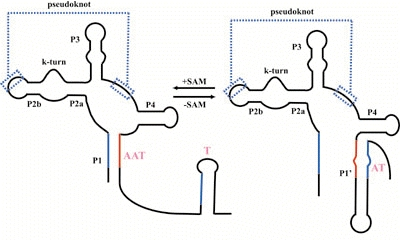
\includegraphics[scale=0.55]{ss-schema}}
\end{center}
\caption{(a) The pipeline for riboswitch structure prediction and binding affinity estimation (b) Schematic of the secondary structure change displayed by the SAM-I riboswitch (The left figure represents the OFF state resulted by the SAM-binding and the right figure represents the ON state)}
\label{fig:ribo-pipeline}
\end{figure}


A brief introduction for the SAM-I riboswitch is presented here, and then we present further details on computational approaches that we plan to use for our scientific goals.  Riboswitches are regulatory RNAs that control the expression of downstream genes. Small metabolite molecules, such as amino acids, nucleotides, coenzymes etc., can bind to riboswitches as effectors in vivo~\cite{mandal}.  In our recent research efforts, the SAM-I riboswitch, one member of the riboswitch family that regulates genes related to the metabolism of sulfur and methionine, has been extensively investigated with atomistic simulations.  This riboswitch choose alternative conformation depending on binding of a S-adenosyl methionine (SAM).  When a SAM is bound, the aptamer domain forms anti-anti-terminator (AAT) conformation, which turns off the downstream genes by forming the terminator (T). Otherwise, the anti-terminator (AT) is formed prohibiting the T element formation for continuing transcription process (see Fig.~\ref{fig:ribo-pipeline}(b)~\cite{brooke}.  Although the structures of the SAM-I riboswitch in the anti-anti-terminator (AAT) conformation have been solved via X-ray crystallography, it is just a static view of how SAM binds to the SAM-I riboswitch RNA.  

Based on our results obtained with extensive all-atom simulations, we became to propose a novel binding mechanism of the SAM-I riboswitch with a SAM in which the role of entropic barrier for the AAT formation as well as the role of $Mg^2+$ specifically bound in the tertiary core structure.  Our results were published in Nucleic Acid Research recently\cite{SAM-I-NAR2009}.  Also, it worth to mention that like the previous years, we collaborate closely with Prof. Fareed Aboul-ela, Biological Science at Louisiana State University, and we expect the results from our computational calculations provide details that are typically inaccessible to experiments; while at the same time providing the opportunity for our simulation results will be validated using biochemical and biophysical experiments (see Fig.~\ref{fig:ribo-pipeline}(a)).   Despite of our success, we face some important questions that should be answered with the proposed simulations and analyses.  First, defying an early assumption, it is increasingly apparent that the interplay between the AAT formation and the AT formation is an important factor to understand the metabolite-assisted folding and consequently gene regulation mechanism with the expression domain.  There are experimental indications from Prof. Aboul-ela lab that the formation of two elements are not exclusive.  Secondly, there exists the fundamental question on how to connect a given sequence with the Riboswitch function such as the binding affinity or the transcriptional efficiency, which could be hinted by characteristic energy landscape features of the sequence. 


\begin{figure}
\begin{center}
  \subfigure[]{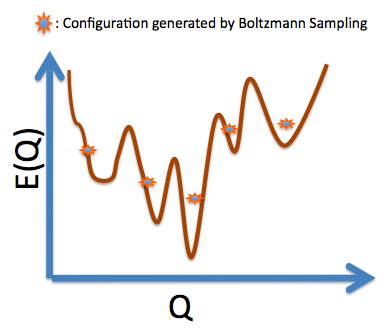
\includegraphics[scale=0.33]{el}}
  \subfigure[]{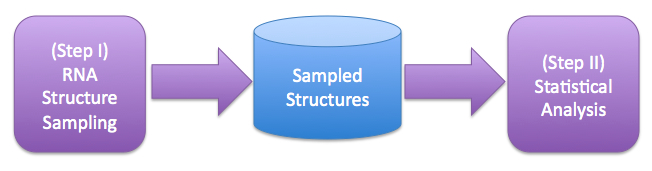
\includegraphics[scale=0.4]{pipeline}}
\end{center}
\caption{(a) Illustration of structure sampling in configuration space.  (b) Schematic of a workflow for sampling and analysis of RNA secondary structures obtained with the Boltzmann-weighted sampling}
\label{fig:folding energy landscape}
\end{figure}

As for simulation costs, major proportion of our allocation will be used for atomistic MD simulations.  Continuing our efforts, the main goal of all atom MD simulations is to probe the dynamic interactions between the SAM-I riboswitch and SAM at the nanoscale and to explore determinants for the specificity. In particular, we aim to examine i) SAM-I riboswtiches and their different constructs that differ from each other in potentially different secondary structures and tertiary interactions, ii) different sequences in SAM-I family, and iii) other SAM riboswiches (SAM-II and SAM-III) for which X-ray structures were recently reported and TPP ribosiwtches that we recently started to investigate.  To estimate binding affinity, we employed the Molecular Mechanics - Poisson Boltzmann Surface Area (MM-PBSA) approach using configuration from MD simulations.  As for efficient sampling of conformational dynamics, replica exchange molecular dynamics (REMD) protocol will be used.  REMD calculations will be carried out using available scripts or with our recent development for the distributed adaptive REMD.  

Basically for all atom simulations, a protocol is similar to one used for previous works.  We could start with a structure derived from the X-ray crystal structures of the AAT conformation of SAM-I riboswitch (PDB: 2GIS, 3GX2, 3GX3, 3GX5, 3GX6, 3GX7)~\cite{montange} or configurations generated by a process via two layers of the pipeline. For a free state riboswitch, SAM is directly removed from the x-ray crystal structure and replaced with solvent water. The amber99bsc0 correction force field is used here~\cite{alberto}. Parameters for SAM are from the Generalized Amber Force Field (GAFF) and missing parameters are calculated using ANTECHAMBER~\cite{wang}. Positions of added hydrogens are guessed using PSFGEN within NAMD 2.6. Then the RNA molecules are solvated in a cubic solvent box of TIP3P waters with a 1.6 nm padding in all directions. Sodium and magnesium ions are distributed around the RNA molecules and neutralize charge of the system. The total number of atoms in the system is 56,000. Energy minimizations are carried out on all of the systems to remove bad contacts. Starting from 0 K, the temperature is raised 10 K for every 10,000 steps and is held constant after reaching the desired temperature (310 K) using temperature reassignment. MD simulations are performed in the NPT ensemble with the pressure maintained using the Langevin piston method with a period of 100 fs and decay times of 50 fs. The time step is 2fs for both equilibration and production phase. Bond lengths between hydrogens and heavy atoms are constrained using SHAKE. The long-range electrostatics is treated with the Particle Mesh Ewald (PME) method with a cutoff distance 1.2 nm.  All MD simulations are carried out by using a parallel version of NAMD 2.6.

\begin{figure}
\begin{center}
  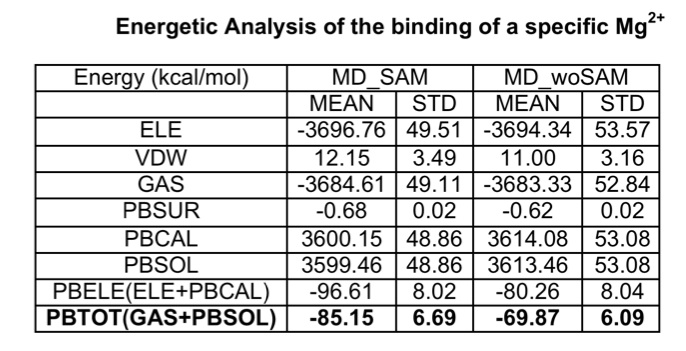
\includegraphics[scale=0.4]{mm-pbsa-mg}
   \caption{MM-PBSA estimation on ${Mg^{2+}}$ binding with a SAM-I riboswitch RNA}
\end{center}
\label{fig:mm-pbsa-mg-table}
\end{figure}

Obtained trajectories will be analyzed with various statistical techniques.  Generally, beyond straightforward trajectory analysis measuring various structural variables, PCA analysis and clustering are useful to extract characteristic dynamical motions in terms of reduced dimension techniques\cite{kimjpcb2010, SAM-I-NAR2009}.   Also, we consider the calculations utilizing the Inherent Structure formalism that might reveal intriguing information with respect to the energy landscape properties such as basins, minima, and saddles\cite{kimpre2002,kimjcp2004}.  Conformational dynamics from obtained trajectories of a complex with a ligand and free state will be used for the MM-PBSA calculation with which ligand binding affinity of the metabolites, SAM, or TPP or other related ligands and also for cation binding of ${Mg^{2+}}$ is estimated.  In particular, ${Mg^{2+}}$ binding has been evidenced as crucial for function of catalytic RNAs but remains as elusive for detailed roles in folding dynamics of riboswitches.  Our preliminary results for cation binding are presented in Fig~\ref{fig:mm-pbsa-mg-table}.  According to our preliminary results, this protocol is useful for ranking ligands that bind a pertinent riboswitch, but also we observed that the accuracy depends on the way for entropy calculation and the use of configurations from MD trajectories.  Also, more challenging questions relevant to the validity of force fields that ignores the polarizability as well as the charge transfer effect should be investigated and we hope our calculations provide interesting clues for the answer.      

In our pipeline approach, the sampling of the Bolzmann ensemble of RNA secondary structures is the primary strategy to explore the energy landscape efficiently.  We use SFold pacakge\cite{ding2006} for the sampling but also consider to develop our own program, in particular, with GPU. The sampling of structures with an input sequence of riboswitches is not computationally intensive, but a considerable number of tasks are required depending on the biological questions.  For example, we carry out comparative investigation to compare all riboswitches of the same family identified in RFam database;,at this moment 2092 SAM-I riboswitches are identified and as the number grows as more genomes are added.  Also, after a sampling step, the analyses are intrinsically many task computing (MTC) tasks (see Fig.~\ref{fig:folding energy landscape}(b)).  
As stated, one notable direction we want to explore with this request is to implement GPU accelerated RNA secondary structure prediction and sampling programs.  We will test our implementation with Lincorn cluster and our request includes computational time with the cluster machine. 


%\begin{figure}
%\begin{center}
%  \subfigure[]{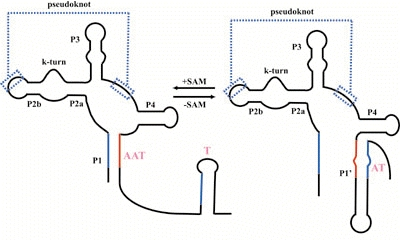
\includegraphics[scale=0.60]{ss-schema}} \hspace{0.05in}
 % \subfigure[]{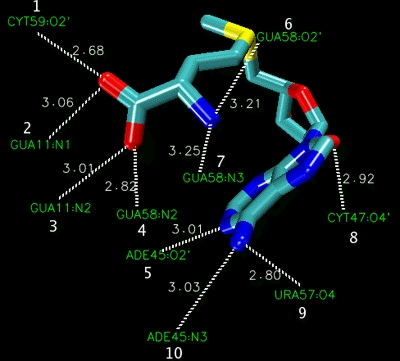
\includegraphics[scale=0.40]{ligand-atom2}}%
%\end{center}
%\caption{(a) Schematic of the secondary structures of s-box riboswitch with SAM bound (left; in the AAT state) and without SAM 
%(right; in the AT state), (b) predicted ligand-SAM interactions with s-box}
%\end{figure}







%All simulations are performed using NAMD 2.6 on LSU (Tezpur) and LONI (Queenbee) Linux clusters. 

%\begin{figure}
%\begin{center}
%   \subfigure[]{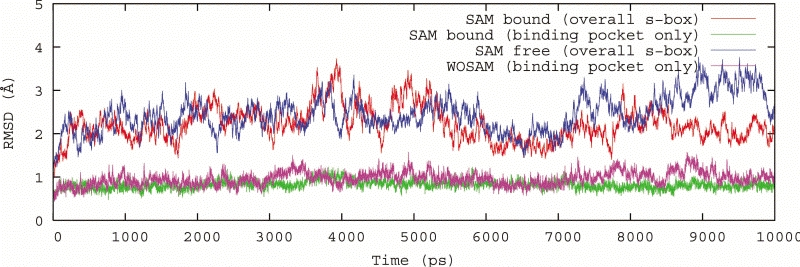
\includegraphics[scale=0.42]{rmsd}} \newline
 %  \subfigure[]{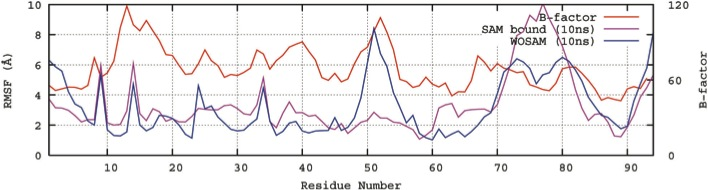
\includegraphics[scale=0.49]{RMSD_residue}}
%\end{center}
%\caption{RMSD of overall s-box and binding pocket only in SAM bound and WOSAM (short for the 
%trajectory of SAM free s-box riboswitch) trajectories  with reference to the crystal structure; (b) Root mean square fluctuation (RMSF) and B-factor of each residue of s-box riboswitch from MD trajectories}
%\end{figure}

%\begin{figure}
%\begin{center}
%   \subfigure[]{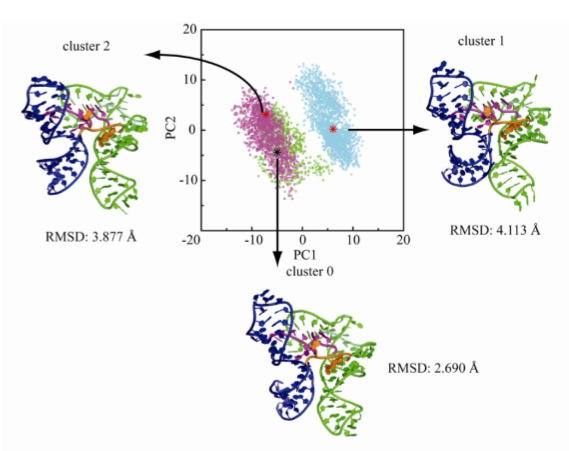
\includegraphics[scale=0.45]{cluster_2D}}
%   \subfigure[]{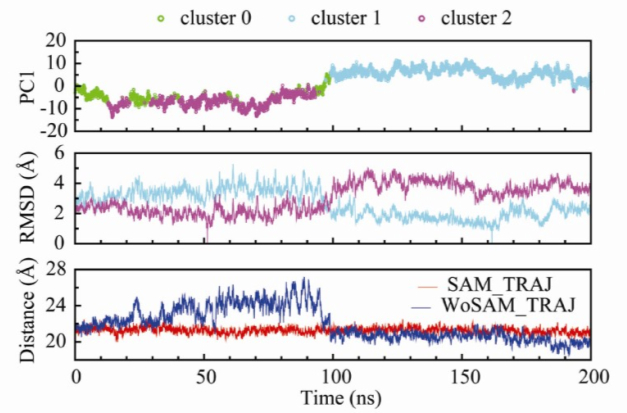
\includegraphics[scale=0.35]{cluster_1D}} \end{center} \caption{Clustering and Principal Component Analysis (PCA) point towards a chopstick-like motion involving P1 and P3 helices in the absence of SAM.  (a) Projections of snapshots of the SAM free trajectory are plotted against the first two principal components and color coded according to a k=3 k-means clustering: cluster 0: magenta, cluster 1, green, cluster 2, magenta. Representative snapshots from each cluster are also shown. This plot indicates that snapshots can be broadly clustered into two groups (cluster 1 and cluster 3) with cluster 2 representing a group with characteristics similar to those of cluster 3. The projection along PC1 broadly separates the clusters, while projection along PC2 completes the separation between clusters 1 and 3. Structures of representative snapshots indicate that clusters are distinguished by a dramatic change in relative position of P1 and P3. (b) From top to bottom: The time evolution of the first principle component of the SAM free trajectory. RMSD for each snapshot in the SAM free relative to the representative snapshots for cluster 1 (cyan curve) and for cluster 3 (magenta curve). The distance between the Center of Mass (COM) of P1 and P3 for the SAM free trajectory (blue) and for the SAM bound trajectory (red).  During the first half of the SAM free trajectory, P1 and P3 helices move apart (clusters 0 and 2), then they move back together during the second half of the trajectory (cluster 1).}

%\end{figure}

%Our initial achievements are illustrated in Figure 5 and Figure 6.  Our results suggest that the presence of SAM in the binding pocket is critical to form P1 helix overcoming the entropic cost for bringing two distal strands in proximity.  The essential dynamics found with the SAM-free trajectory are shown in Figure 6 with clustering results, indicating the characteristic long time dynamics in the SAM-free system. 




%\begin{figure}
%\begin{center}
%  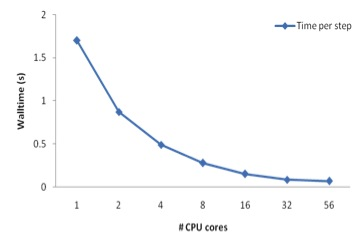
\includegraphics[scale=0.660]{56k_scaling-2} \caption{Wall-clock times taken (in second) for each step at different processor counts. The measurement was done with Queen Bee }
%\end{center}
%\end{figure}


\begin{table}[h]
\begin{center}
  \caption{Riboswitch simulations and expected computing resources. \jhanote{Please update} }
\label{table:systems}
\begin{tabular}{| c | c | c | c |}
\hline
Type of Calculation &   Method or Package  &    HPC resources to be used & SUs required \\
\hline \hline
RNA secondary structure &
Sfold/RNAfold& Ranger (34 K) & 100K\\ 
sampling and analysis  & /our developed program  & /QB (33 K) /Abe (33 K) & \\  \hline
Atomistic MD simulation & NAMD  & Ranger (300 K) /QB (100 K)  & 850K \\  
MM-PBSA        & AMBER    & /Abe (200 K)/Kraken (250 K) &  \\ \hline
RNA secondary structure & In -house CUDA code & Lincorn & 50K \\
 sampling and analysis &   
&  &  \\
\hline
\end{tabular}
\end{center}
\end{table}

\subsubsection*{Requested Computational Resources}

As for all-atom MD simulations, according to our benchmark with Queen Bee, when using 32 cores, the time taken per step is approximately 0.06s for the simulation system of a SAM-I aptamer RNA described above; thus the wall clock time required to complete 1ns is .34 day; in other words for a 56K system, 1 ns simulations require $\approx$ 300 CPU hours.  Thus each 100 ns simulation requires approximately 30,000 CPU hrs.  Since our simulation results indicated that more than 300 ns trajectory is desirable for observing meaningful conformational dynamics. Therefore, without additional post-analyses including MM-PBSA calculations, we expect simulations of about 90 trajectories with 850,000 SUs (See {\url{http://staging.teragrid.org/userinfo/aus/namd_benchmark.php}} ).  As for RNA secondary structure calculations, our test calculation for 2092 sequences takes 6 CPU hours with 32 cores for Boltzmann Enesmble sampling.  And, analyses require 10-100 times of sampling time.  Therefore, we expect to consume 100 K SU for 5 - 50 calculations that combine the sampling and the analyses.  Finally, we request 50 K with Lincorn cluster only for testing purpose of our GPU implementation.  




\section*{Project 3: Atomistic Simulations of Physiological Systems}

\subsection*{Project 3a: Towards patient specific HIV therapy}
%\begin{compactenum}[a)]

\emph{Scientific objectives: } The long term scientific objective of our project is to develop molecular dynamics simulations of HIV-1 Pol enzymes into a tool for clinicians to use in determining the cocktail of drugs to administer to an HIV-infected individual. This work is supported by grants under EU FP7 and FP6 via the VPH-NOE (EU FP7-ICT-2007-5.3 223920), Contra Cancrum (EU FP7-ICT-2007-5.3 223979) and Virolab (EU FP7 223131) projects. For such applications, reproducible accuracy at the level which can rank drug efficacies, and rapidity of acquisition of results (for clinical relevance) are all essential. This takes the application of bio-MD techniques into an entirely new domain.

We have developed an automated protocol to perform simulations and calculate binding affinities in the case of the protease (PR) enzyme\cite{Stoica2008} which we have recently enhanced based on the discovery that ensembles of short simulations produce better sampling than single long timescale simulations\cite{Genheden2009,Sadiq2010}. Molecular dynamics simulations require a crystal structure from which to start, but there will always be far less structures than there are HIV \emph{pol} genotypes. Therefore we need to ensure that we can computationally mutate a crystal structure into any desired 
genotype whilst still accurately calculating binding energy values. Our recent work has successfully reproduced the experimental binding free energy ranking of a series of multiply drug resistant (MDR) mutants of increasing resistance (see Table \ref{tab:mutations}) to the inhibitor lopinavir (LPV) as published by Ohtaka \emph{et al.}\cite{Ohtaka2003}. This selection of six PR sequences will be refered to as the MDR genotype set in the rest of this document. Our next aim is to validate the use of our simulation and analysis protocol by reproducing the results for the other five FDA approved inhibitors included in this study (a list of the inhibitors included is given in Table \ref{tab:inhibitors}).

\begin{table}[h! b! p!]
\begin{center}
\begin{tabular}{ l  l  l }
\textbf{Sequence Code} & \textbf{Description} & \textbf{Mutations}\\
\hline
\textbf{WT} & Wildtype & HXB2\\
\textbf{HM} & MDR hexa-mutant & L10I, M46I, I54V, V82A, I84V, L90M\\
\textbf{QM} & MDR quatro-mutant & M46I, I54V, V82A, I84V\\
\textbf{AS} & Active site mutant & V82A, I84V\\
\textbf{FL} & Flap mutants & M46I, I54V\\
\textbf{DM} & Dimer interface mutants & L10I, L90M\\ 
\hline
\end{tabular}
\end{center}
\caption{Codename and mutational composition of HIV-1 protease sequences investigated.}
\up
\label{tab:mutations}
\end{table}

\begin{table}
\begin{center}
\begin{tabular}{l l}
\textbf{Inhibitor Code} & \textbf{Inhibitor Name}\\
\hline
APV & amprenavir\\
IDV & indinavir\\
LPV & lopinavir\\
NFV & nelfinavir\\
RTV & ritonavir\\
%\textbf{SQV} & \textbf{saquinavir - Better to Remove?}\\
\hline
\end{tabular}
\end{center}
\caption{Code and full names of the HIV-1 protease inhibitors investigated.}
\up\up
\label{tab:inhibitors}
\end{table}

In the last year we have expanded our protocol to include the reverse transcriptase (RT) enzyme and the Non-Nucleotide Reverse Transcriptase Inhibitor (NNRTI) class of drugs for which the required system is more than 3 times larger than PR (solvated RT systems contain 180,000 atoms compared to 50,000 for PR). Our work indicates that the effects of active site mutations can be successfully descriminated using enzyme bound simulations alone (as we do in the protease case), without the need for additional simulations of the apo enzyme. Our intention is to study the inhibitors efavirenz (EFZ) and nevirapine (NVP) bound to wildtype, Y181C, L100I and K103N single mutants, the L100I/Y181C and L100I/K103 double mutants and the L100I/K103N/Y181C triple mutant RT sequences. Our previous work focussed on the L100I and K103N mutations but we have now added the Y181C mutation to this set. Unlike the previous mutations, this gives differing levels of resistance to EFZ and NVP (according to the Stanford database - http://hivdb.stanford.edu/pages/algs/HIVdb.html). Along with calculating the binding free energies of the ligand-bound enzymes, we also intend to extend the individual simulations to investigate the impact of these mutations on the rigid body motions between the fingers and thumb subdomains of the p66 subunit of RT. A recent molecular dynamics study shows that NVP operates as a molecular wedge constraining these catalytically important protein motions\cite{Ivetac2009}. This work indicates that our simulations will need to be of order of at least 30ns in length in order to observe the appropriate properties; along with the evidence from our previous work that free energies calculated for RT simulations vary less than those of PR this informs our decision to perform ensemble-based calculations containing fewer replicas but of longer duration. This second line of investigation provides further justification for including the Y181C mutation as, by replacing the bulky tyrosine residue with the smaller cysteine, a much larger perturbation of the binding pocket geometry is produced which might be expected to invoke more marked alterations in the motions of the fingers and thumb domains.

\emph{Computational Requirements: } We have performed our simulations via the widely used molecular dynamics package NAMD \cite{Phillips2005} with the AMBER \cite{Case2005} suite of MD routines used to parameterise the models prior to simulation and then to analyse the resultant trajectories and calculate the free energy ($\Delta$G) values. In addition to these packages in our future work we plan to use the Nucleic Acid Builder module of AMBER on TeraGrid resources in order to compute the entropy changes via normal mode analysis for the RT system.

Previous work on Ranger benchmarked at 7 hours wallclock time per nanosecond on 32 cores for the protease system and 6.5 hours per nanosecond on 128 cores for reverse transcriptase. These values have been used to estimate the required SUs in Table \ref{t:hiv_req}. We have recently gained access to the Kraken system and have benchmarked the protease system to take 5 hours per nanosecond which, combined with the fast turn-around times, makes Kraken an appealing platform upon which to run our simulations.

The disk requirements for all of the simulations listed in Table \ref{t:hiv_req} will not be required simultaneously; at any
one time it will not exceed 5TB. The majority of this data is *.dcd formatted trajectories output as simulations progress which can be archived once analysis has been completed. The trajectories can be transferred quickly between the TeraGrid and our local storage making use of the optical fibre network infrastructure. We currently have access to 6TB of storage at UCL (UK) and also make extensive use of the Ranch archiving system available at TACC.

\begin{table}[h]
\centering
\begin{tabular}[b]
{|>{\scriptsize}c|>{\scriptsize}c|>{\scriptsize}
c|>{\scriptsize}c|>{\scriptsize}c|>{\scriptsize}c|>{\scriptsize}c|}
\hline
\textbf{Sim Description} & \textbf{No. Sims} &
\textbf{No. Cores} & \textbf{Disk} &
\textbf{Code} & \textbf{TG machine} & \textbf{Total SUs}\\
\hline
\multicolumn{7}{|c|}{\textbf{PR Multiple Drug Resistance Study}}\\
\hline
APV - 6 MDR systems & 400 & 32 & 250GB & NAMD & Ranger & 448,000 \\
\hline
IDV - 6 MDR systems & 400 & 32 & 250GB & NAMD & Ranger & 448,000 \\
\hline
NFV - 6 MDR systems & 400 & 32 & 250GB & NAMD & Ranger & 448,000 \\
\hline
RTV - 6 MDR systems & 400 & 32 & 250GB & NAMD & Ranger & 448,000 \\
\hline
\multicolumn{7}{|c|}{\textbf{RT Drug Resistance Study}}\\
\hline
RT Wildtype EFZ & 10 & 128 & 300GB & NAMD & Kraken & 208,000\\
\hline
RT L100I EFZ & 10 & 128 & 300GB & NAMD & Kraken & 208,000\\
\hline
RT K103N EFZ & 10 & 128 & 300GB & NAMD & Kraken & 208,000\\
\hline
RT Y181C EFZ & 10 & 128 & 300GB & NAMD & Kraken & 208,000\\
\hline
RT L100I/K103N EFZ & 10 & 128 & 300GB & NAMD & Kraken & 208,000\\
\hline
RT L100I/Y181C EFZ & 10 & 128 & 300GB & NAMD & Kraken & 208,000\\
\hline
RT L100I/K103N/Y181C EFZ & 10 & 128 & 300GB & NAMD & Kraken & 208,000\\
\hline
RT Y181C NVP & 10 & 128 & 300GB & NAMD & Kraken & 208,000\\
\hline
RT L100I/Y181C NVP & 10 & 128 & 300GB & NAMD & Kraken & 208,000\\
\hline
RT L100I/K103N/Y181C NVP & 10 & 128 & 300GB & NAMD & Kraken & 208,000\\
\hline
Grand total of SUs required & & & & & & 3,872,000\\
\hline
\end{tabular} \caption{Planned simulations and associated computational requirements.}
\label{t:hiv_req}
\up\up\up
\end{table}
%\end{compactenum}
      


\subsection*{Project 3b: Predicting the affinity of the EGFR kinase domain for drug inhibitors of lung cancer}
%\begin{compactenum}[a)]
\emph{Scientific objectives: } The epidermal growth factor receptor (EGFR) is an especially important enzyme target in lung cancer therapy because it mutates and/or is overexpressed in most non-small cell lung carcinoma (NSCLC) tumours. Inhibition of kinase activation of EGFR is a frequently used method to suppress its functions \cite{bib:nature_tki}. The majority of tyrosine kinase inhibitors (TKIs) are ATP-competitive inhibitors which bind in the ATP-binding site. Molecular dynamics (MD) simulations will be used to study the structural and energetic properties of inhibitor-EGFR complexes. The binding affinity of inhibitors to EGFRs will be calculated by molecular mechanics Poisson-Boltzmann surface area (MM/PBSA) methods \cite{bib:wan_philtrans}. This molecular level study is one component of the EU FP7 ContraCancrum (Clinically Oriented Translational Cancer Multilevel Modeling) project which aims at developing a composite multilevel platform for simulating malignant tumor development and pharmacologic responses to a therapeutic intervention (http://www.contracancrum.eu). We have employed large scale MD techniques using both TeraGrid and DEISA resources in order to study the interactions of inhibitors with wild-type and mutant EGFRs \cite{bib:wc2009}. A better understanding of the reasons for the success or failure of a therapeutic intervention will help us in the selection of subgroups of patients who are most likely to respond to specific drugs, and paves the way for personalized treatment \cite{bib:hiv}. We have already performed a preliminary study of different inhibitors (AEE788, AFN941 and gefitinib) with EGFR which we now intend to extend to look at a wider variety of inhibitors and EGFR mutations and to probe longer time scale motions of the protein.

%\item \emph{Benchmark Data}
%\begin{comment}
%\begin{figure}
%\centering
%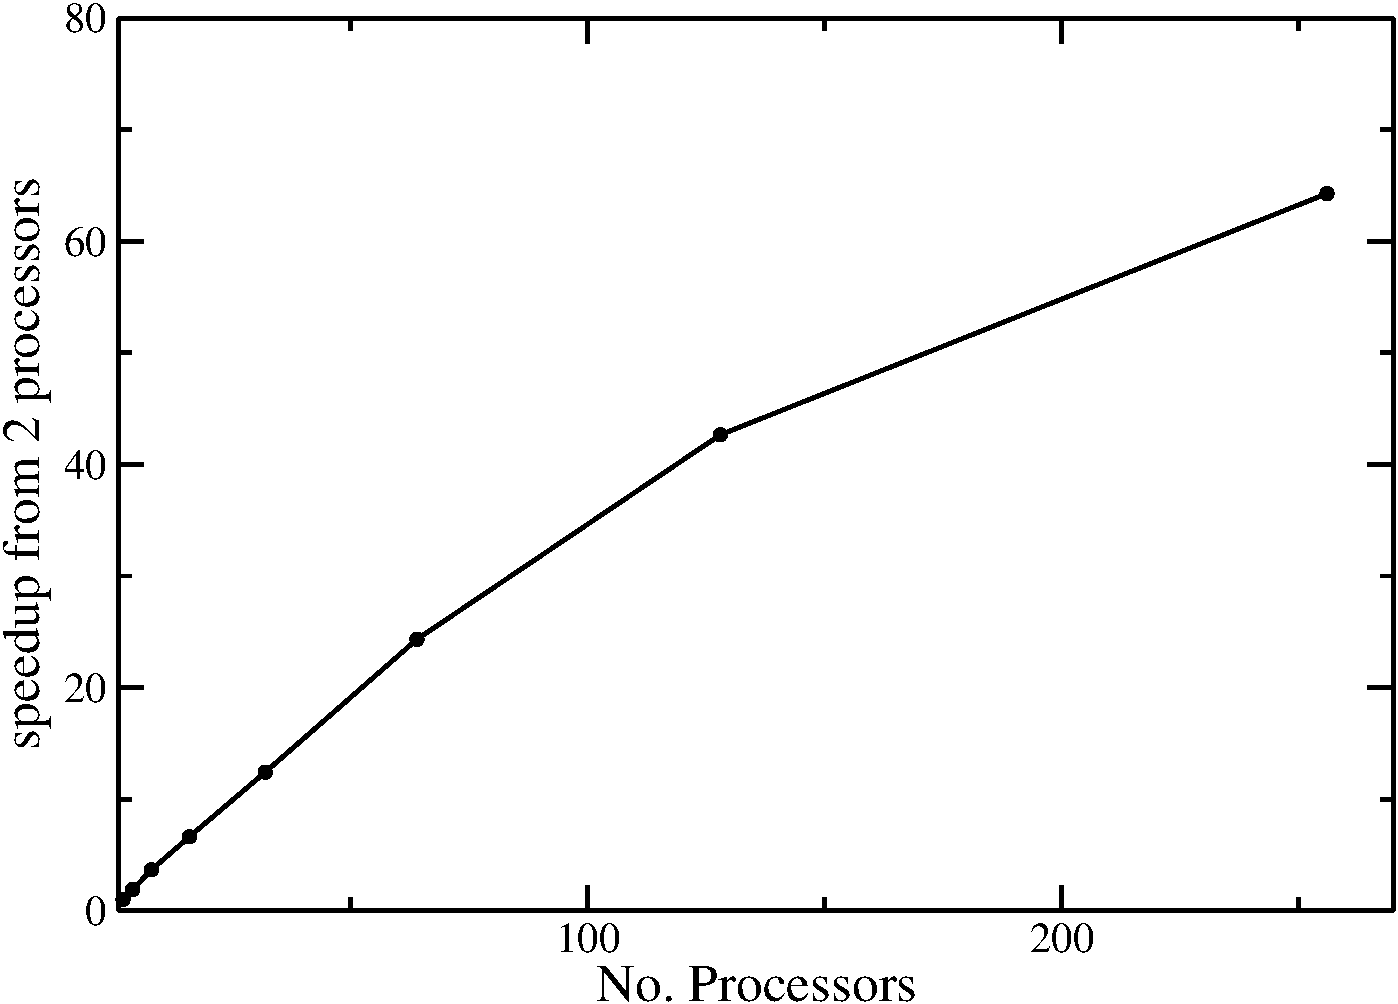
\includegraphics[scale=0.5]{efgr/benchmark}
%\caption{Benchmark of NAMD simulations for inhibitor-EGFR system}\label{fig:benchmark}
%\end{figure}
%\end{comment}
%Based on our benchmark study on Ranger (see Figure VIII of the attached `Benchmark Document'), 
%and preliminary simulations, each simulation will run optimally on 128 processors, 
%and it will consume 300 SUs/ns.
%Based on our benchmark study on Ranger (Figure \ref{fig:benchmark}), and preliminary simulations, each simulation will run optimally on 128 processors, and it will consume about 300 SUs/ns.

\emph{Resource requested:} Computational requirements on Ranger for intended studies of EGFR-inhibitor interaction are listed in Table \ref{t:efgr}.

\begin{table}[h]
\centering
\begin{tabular}[b]
{|>{\scriptsize}c|>{\scriptsize}c|>{\scriptsize}
c|>{\scriptsize}c|>{\scriptsize}c|>{\scriptsize}c|>{\scriptsize}c|}
\hline
\textbf{Sim Description} & \textbf{No. Sims} &
\textbf{No. Cores} & \textbf{Disk} &
\textbf{Code} & \textbf{TG machine} & \textbf{Total SUs}\\
\hline
AEE/EGFRs (50,000 atoms) & 50$^a$ $\times$ 25$^b$ & 128 & 100GB & NAMD & Ranger & 2,000,000\\
\hline
Erlotinib/EGFRs (50,000 atoms) & 5$^c$ $\times$ 50$^a$ $\times$ 1$^b$ & 128 & 100GB & NAMD & Ranger & 400,000\\
\hline
Grand total of SUs required & & & & & & 2,400,000 \\
\hline
\end{tabular} \caption{Planned simulations and associated computational requirements. $^a$Number of replicas in one ensemble simulation; $^b$Number of simulations for each replica, each simulation lasts for 4ns; $^c$Wild-type and 4 mutant (G719S, L858R, T890M and T790M/L858R) EGFRs.}
\label{t:efgr}
\end{table}
%\end{compactenum}



\section*{Project 4: Large-scale molecular dynamics simulations of layered bio-mineral composites}
 %\begin{compactenum}[a)]
\emph{Scientific objectives:} The objective of this work is to %calculate the properties of clay platelets immersed in a polymer matrix (a nanocomposite system) and to 
investigate the complex interaction between bio-molecules and clay-mineral systems relevant to origins of life and applications to drug delivery. 
This work is supported by UK EPSRC RealityGrid Platform Grant (EP/C536452/1), 
an EPSRC PhD studentship and the UK Technology Strategy Board's NIMES (Q2506L) project.
Hitherto, research into the origins of life has rarely used simulation techniques to understand the possible chemical pathways to the formation of early bio-molecules. The main purpose of this research is to use computer simulation to provide insight into the structure, conformation and stability of nucleic acids while interacting with a clay surface, both intercalated between the layered minerals and adsorbed onto the edge of the layered mineral. Such insight is difficult to obtain experimentally due to the disordered nature of these systems. From the increased computational power of the TeraGrid, it is possible to effectively model realistic sized fully atomistic models which can simulate an aqueous clay surface and incorporate large bio-molecules, such as ribozymes, whilst removing finite size effects \cite{JPCC_2007}. It is also now possible to access timescales in the range of hundreds of nanoseconds where previously only tens of nanoseconds were accessible, in conceivable real-time. These increased timescales are particularly relevant for large complex nucleic acid (RNA \& DNA) molecules in which folding of the molecule into functional tertiary structures happens over long timescales. 

In nature, clay materials are composed of platelets approximately 1
micrometre wide and, in  bio- and non-bio composites, these platelets are dispersed in a matrix of 
polymer chains.  In conventional molecular dynamics simulations of nanocomposites, a small simulation cell is replicated to represent an infinite clay platelet. This is an approximation that we have started to remove in our studies and will now apply to biomolecular -clay systems, by creating very large clay systems which can accommodate large complex bio-polymers, and also by examining isolated clay platelets, with edges, of realistic size. 

In an extension to our previous bio-clay nanocomposite work, we plan to explore the mechanism by which RNA adsorbs on external aqueous montmorillonite mineral surfaces, using molecular dynamics (MD) techniques, to look at the interaction of RNA of differing base sequences with the mineral surface in the presence of differing charge balancing cations. This will give a molecular level understanding of the mechanism by which RNA adsorbs/interacts with the montmorillonite surface to support experimental findings of these systems \cite{Franchi, Huang}. Other work will look at the relative structural stability of free and layered Mg-Al double hydroxide intercalated nucleic acids, at temperatures and pressures relevant to origins of life studies, see Figure \ref{F:pics} (contained within this document). For both clay systems we will firstly study the interaction of RNA intercalated within the clay framework (i.e. the basal surface).  From these simulations it will be possible to calculate the mean-squared displacement and the radius of gyration of the bio-molecule as well as finding the dominant modes of motion through principal component analysis. Radial distribution functions, atomic density profiles and time-averaged visualizations of the systems will provide the structure and conformation of the whole system.
 
\begin{figure} 
        \begin{center}
           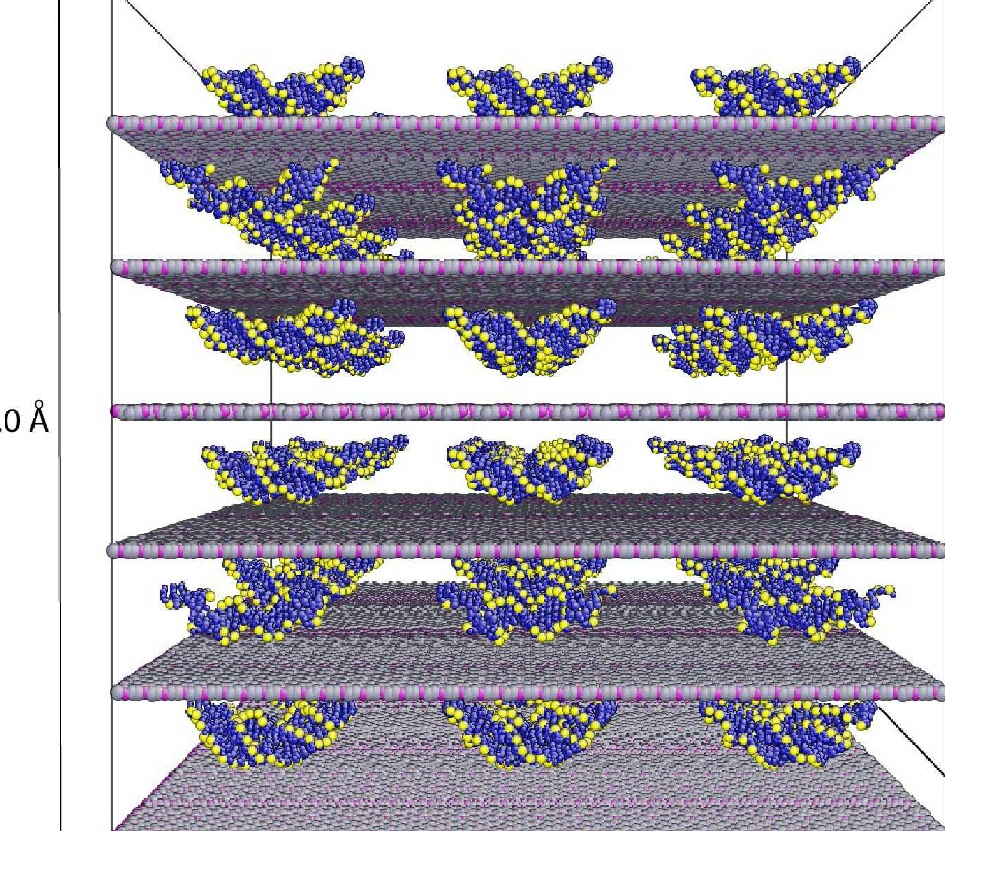
\includegraphics[scale=0.3]{subproject1-bioclays/pic1}
           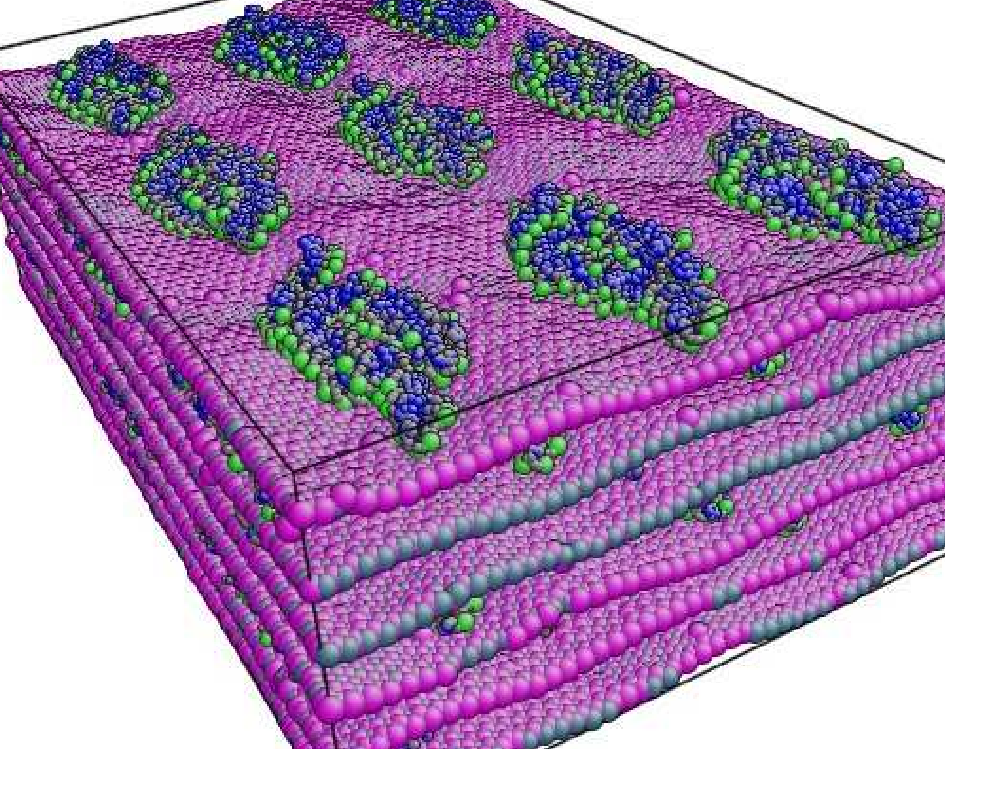
\includegraphics[scale=0.3]{subproject1-bioclays/pic2}
           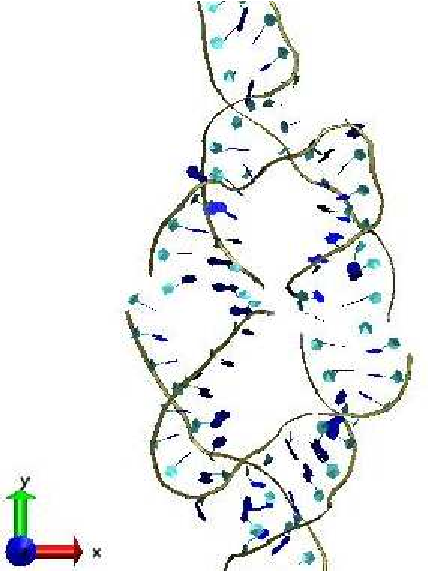
\includegraphics[scale=0.3]{subproject1-bioclays/pic3}
        \end{center}
%\caption{Visualizations of a hammerhead ribozyme intercalated into an LDH clay mineral consisting of 1,181,736 atoms.}
\caption{Initial stucture of the hammerhead ribozyme intercalated into an LDH clay mineral at the 
start of simulation (a) consisting of 1,181,736 atoms.  Magnesium, aluminium, chlorine, phosphorus, 
carbon and nitrogen atoms are represented as light grey, pink, green, yellow, dark grey and blue 
spheres respectively. (b) Final stucture of the large LDH-ribozyme model after the 3.5ns 
production phase of simulation.  Magnesium, aluminium, chlorine, phosphorus, carbon and nitrogen 
atoms are represented as light grey, pink, green, yellow, dark grey and blue spheres respectively.  
All nucleotide motion within the LDH sheets is significantly restricted compared to that in 
bulk water. In addition, visualisation reveals properties such as thermal undulations in the LDH 
sheet, as well as corrugation of the layers around the nucleotides. (c) Visualisation of the ribozyme 
molecule after 3.5ns of simulation, using ribbon notation.}
\label{F:pics}
\end{figure}

%To Each model will include several dispersed ($Na^{+}$ montmorillonite) platelets immersed in either i) a matrix of poly(ethylene glycol) polymer  and ii) large biomolecules such as RNA in aqueous solution. 
%From these simulations will we perform several non-equilbrium molecular dynamics simulations (NEMD), from which we will  calculate material properties, including the bending modulus, Young's
%modulus and Poisson's ratio. %We will also be able to study the interactions between seperate platelets, which may determine the rheology of clay nanocomposites .  It is the increased mechanical and
%thermochemical stability of clay-polymer nanocomposites that has
%received much attention recently in a variety of industries
%\cite{Pinnavaia_book}; 
%our objective is to gain a greater understanding of this enhancement through these
%
%simulations. 
Secondly, we will consider the adsorption of smaller RNA molecules on the edge of clay platelets. 
This will give us insight into the mechanism of
intercalation in these compounds, required for understanding their formation. This is important not just for origins of life studies, but also in the processing conditions for drug delivery applications~\cite{understanding}. For example, we will be able to see changes in the clay sheet conformation that occur with initial intercalation of the bulky biopolymers, such as the layers moving apart from each other, and whether the flexibility of the clay sheet plays a significant role. 

To approach a realistic sized platelet for long simulation times, we require system sizes 
of order 1 - 20 million atoms. The largest system will include several isolated platelets of 
realistic size with biopolymers interacting with the clay sheet edges. This size of simulation 
is now firmly within the mesoscopic regime but simulated in full atomistic detail. We shall 
include non equilibrium simulations to simulate the conditions required for the bulky biopolymers 
to intercalate between the clay sheets on a timescale we can observe with atomistic molecular 
dynamics. These non-equilibrium conditions include compressive stress and shear, which effectively 
force the biopolymers into the clay interlayer region.
%To approach a realistic sized platelet for the long simulation times, we require system sizes of order 1 - 20 million atoms. The largest system will include several isolated platelets of realistic size with biopolymers interacting with the clay sheet edges. This size of simulation is firmly within the `mesoscopic' regime but simulated in full atomistic detail. We shall include non-equilibrium simulations to understand the response of these systems to compressive / extensive stress and under shear. 

%\textbf{Principal scientific objectives} We aim to calculate the
%structural, dynamical and materials properties of a clay platelet
%($Na^{+}$ montmorillonite) immersed in a matrix of poly(ethylene glycol)
%directly from large scale molecular dynamics simulations.
% Additionally  The mechanism of intercalation in clay-polymer
%nanocomposites is unknown, and this will provide valuable
%insight.

%\item\emph{Previous Work on the TeraGrid}
%Publications and progress made in the past year on TG resources.
%In our previous simulations we utilized periodic
%boundaries on the clay sheets, allowing a simulation cell to represent
%an infinite clay platelet \cite{JPCC_2007,Thyveetil,Thyveetil_JACS, Soft_Matter1}.  
%These large-scale, fully atomistic
%simulations, 
%approached the size of a physically realistic platelet.
%From
%this, we were able to calculate mesoscopic and macroscopic properties
%directly from  molecular dynamics simulations in the absence of
%finite-size effects of both clay nanocomposites\cite{JPCC_2007,Thyveetil, Soft_Matter1} and bio-%composites~\cite{Thyveetil_JACS}.

%Using the last LRAC allocation we extended these simulations to calculate 
%the mechanical response of poly(ethylene oxide) polymer-clay nanocomposites, 
%separating the response into contributions from the polymer and clay 
%mineral layer~\cite{Soft_Matter1}. This separation technique allowed us 
%to determine how the clay-polymer elastic properties change with distance 
%from the clay surface. This is the first time the effect of mineral layers 
%on the elastic modulus of polymeric materials in the vicinity of a mineral 
%surface has been calculated. This result is a vital first step to 
%understanding the enhancement mechanism of nanocomposites and the role of 
%the very large surface area of the clay mineral layer on the surrounding medium. To simulate a 
%realistically sized clay platelet required very large scale simulations, made possible using the resources available via 
%the LRAC allocation. 

%We have also examined the mechanisms by which clay mineral layers buckle in clay-polymer nanocomposites under compressive stress. We find that a clay sheet remains stable in a flat state until a critical compressive strain is reached, at which point it buckles, and regains its uncompressed area. Over this buckling transition, the Poisson ratio of the clay sheets turns negative, a property which has been predicted for 2-dimensional sheets ~\cite{Soft_Matter2}. This is the first time such behaviour has been seen in a molecular simulation of mineral layers. The large scale allowing us to probe large buckling wavelengths that are inhibited in smaller scale simulation. 

%We have explicitly included the edges of the clay sheets with the clay platelet completely surrounded by water (Figure~\ref{Fig:water}). The clay platelet consists of  two sheets of $Na^{+}$ montmorillonte clay, which are either aligned or 
%staggered relative to each other in two different models.  
%In long MD simulations, we have observed ingress into the intersheet spacing by water, which is only possible when edges are explicitly included.  We are currently analysing the diffusional properties of the water inside the clay interlayer and the effect on the clay dynamical properties, such as clay sheet thermal undulations. 
%This has never been done before either by simulation or experiment. 
%\begin{figure}
%        \begin{center}
%           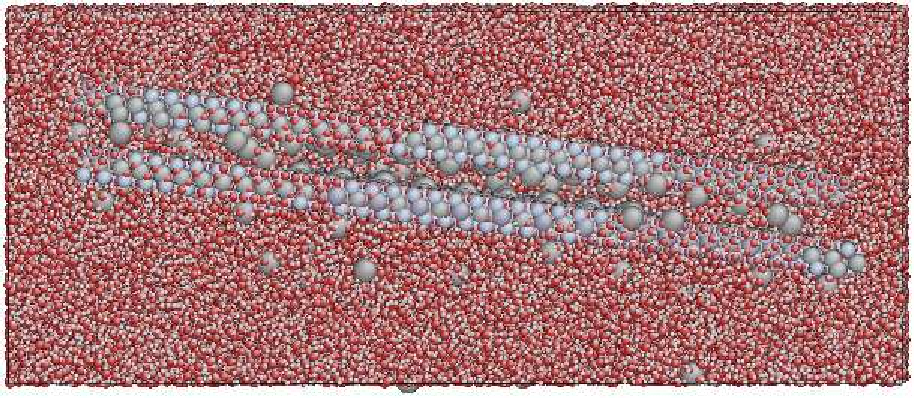
\includegraphics[scale=0.6]{subproject1-bioclays/ymod}
%        \end{center}
%\caption{Visualization of the ingress of water into an isolated clay platelet; the viewpoint is a slice through the clay sheet. Light grey and light blue atoms are the silicon and aluminium atoms of the clay sheet respectively. Oxygen atoms are coloured red and hydrogen atoms are coloured white. Sodium ions, located in the clay interlayer, are dark grey. We can see some sodium ions move away from the surface as the water diffuses through the clay interlayer. }
%\label{Fig:water}
%\end{figure}
% Our previous studies, with periodic boundaries on the clay sheets themselves, were 2/3
%orders of magnitude larger than any previous atomistic simulations of
%clay minerals. They revealed the clay sheets to have some degree of
%flexibility, manifesting as long range, low amplitude undulations with
%wavelengths greater than 25 nm, which are only revealed through
%large scale simulations \cite{jls_2006,thyveetil2007}.  %As an extension 
%to the previous study, we will explicitly include the edges of the 
%clay sheets and the platelet will be completely surrounded by the 
%polymer matrix. The clay platelet will
%consist of  two sheets of $Na^{+}$ montmorillonte clay, which will be
%aligned and staggered relative to each other in two different models.  We
%shall compare the structural and dynamical properties of both the polymer
%and clay platelet to conventional molecular dynamics simulations of
%clay-polymer nanocomposites \cite{cmj_12}.

%\item \emph{Code to be used}
%We will use the scalable molecular dynamics code, LAMMPS \cite{LAMMPS, LAMMPS_2005}, to perform these
%simulations. We will use the rRESPA multi-timestep method \cite{rRESPA} combined with the efficient particle-particle-particle-mesh method \cite{Hockney_book} to calculate the electrostatics. 


%\item \emph{Benchmark Data}
%We have performed comprehensive benchmarks of 
%a hydrated montmorillonite system up to 85 million atoms on Ranger and Kraken.
%See Figure V of the attached `Benchmark Document' for scaling data.

%We find approximately linear scaling up to 2048 processors for 10 million atoms, and up to 4096 for 85 million atoms on Ranger; and up to 2048 for 100 million atoms on Kraken.

\emph{Resource requested:} The simulations to be performed and associated computational requirements are listed in Table \ref{t:claytable}. Each simulation listed of the biopolymer interacting with clay edges will run for 20ns; simulations of the bio-clay systems on the basal clay surfaces will be run for 100ns, to ensure correct conformational sampling of the highly flexible biomolecules is achieved.
 
\begin{table}[!h]
\centering

\begin{tabular}[b]
{|>{\scriptsize}c|>{\scriptsize}c|>{\scriptsize}
c|>{\scriptsize}c|>{\scriptsize}c|>{\scriptsize}c|>{\scriptsize}c|}
\hline
\textbf{Sim Description} & \textbf{No. Sims} &
\textbf{No. Cores} & \textbf{Disk} &
\textbf{Code} & \textbf{TG machine} & \textbf{total SUs}\\
\hline 
Clay edge simulations &  10 & 4096 & 2TB & LAMMPS & Ranger & 2,000,000  \\
\hline
NEMD clay edge simulations & 40 & 4096 & 4TB & LAMMPS & Ranger & 1,000,000 \\
\hline
RNA montmorillonite &  15  & 2048 & 1TB & LAMMPS & Kraken & 500,000 \\
\hline
nucleic-acid LDH & 30 & 2048 & 2TB & LAMMPS & Kraken & 750,000 \\ 
\hline
Grand total of SUs required & & & & & & 4,250,000  \\
\hline
\end{tabular} 
\caption{Summary of biopolymer clay simulations and
simulation times for jobs to be run on Ranger (simulations containing clay edges) and Kraken (interlayer bio-clay composites).}
%\caption{Planned simulations of hydrated
%PEG/$Na^+$-montmorillionite on Ranger 
%(simulations containing clay edges) and Kraken (bio-clay composites).}
\label{t:claytable}
\end{table}
%\end{compactenum}
      



\section*{Project 5: Expeditions in Distributed Computing using SAGA}

\jhanote{Yaakoub-- Please take a first shot. Include resource request for LINCOLN. Please also update
with some details of the TG10 paper submission.}

Advances in Grid applications have simply not kept pace with advances in other aspects of 
distributed CyberInfrastructure, such as Grid middleware -- whether measured by the number of 
existing applications that can easily utilize the many advanced features offered by distributed 
infrastructure or measured by the number of novel applications capable of using the 
infrastructure. A key impediment in the accelerated development and deployment of Grid 
applications is the scarcity of high-level application programming abstractions that bridge the 
divide between the needs of Grid applications and the capabilities offered by middleware.  Much 
Grid development has focused on the support for legacy parallel and cluster application codes 
as a way of ensuring scientific relevance.  The benefit of the Grid paradigm, however, will 
come from new application development that does not depend on the homogeneous and relatively 
static model of resource performance inherited from parallel or cluster legacies.  % The lack 
%of such application-level programming abstractions is compounded by the fact that there exist 
%incompatible and often changing Grid middleware systems in both research and production 
%environments.

To address these challenges and in particular to find a solution to the universal, apparently 
intractable problem of successfully Grid-enabling applications, several applications groups 
expressed the desire for a simple programmatic interface that is widely-adopted, widely-available 
and usable. The goal of such an interface would be to provide a ``grid counterpart to MPI'' (at 
least in impact if not in details) and that would supply developers with a simple, uniform, and 
standard programmatic interface with which to develop distributed applications.  Thanks to the 
efforts of many contributors, but in particular the PI's group, an initial specification of 
such a ``grid counterpart to MPI'' now exists -- the Simple API for Grid Applications 
(SAGA)~\cite{saga_url}. As of fall 2010, SAGA will be an Open Grid Forum (OGF) technical 
specification.


\subsection*{Project 5a: Developing and Deploying Applications using SAGA}

A wide range of applications have been developed using SAGA -- ranging from regular compute 
intensive applications but involving multiple resources ~\cite{saga_escience07, gmac, REMD-
PhilTranA2009}, applications with multiple components and possibly irregular runtime 
requirements~\cite{saga_loosely_coupled, teragrid08} as well data-intensive applications 
~\cite{saga_data_intensive, saga_grid_cloud} using programming abstractions such as 
MapReduce~\footnote{Implementation of MapReduce using SAGA is funded by Google} An initial 
prototype of a ``general pilot-job'' framework using SAGA that can be utilized for Replica-Exchange 
that enables the {\it trivial} utilisation of multiple distributed resources across TeraGrid has 
been developed. This is currently work in progress, but we anticipate sufficient progress to begin 
testing the framework using our 56K riboswitch model.~\cite{REMD-PhilTranA2009}. %A Brief schematic 
%of Distributed Adaptive Replica Exchange Molecular Dynamics is shown in Figure 8.
Our current framework implements the Generalized Pilot-Job feature with the BigJob abstraction 
built upon SAGA and utilization of the framework is the key component for successful massive REMD 
simulations for our project on riboswitch studies.

\begin{figure}
\begin{center}
\subfigure{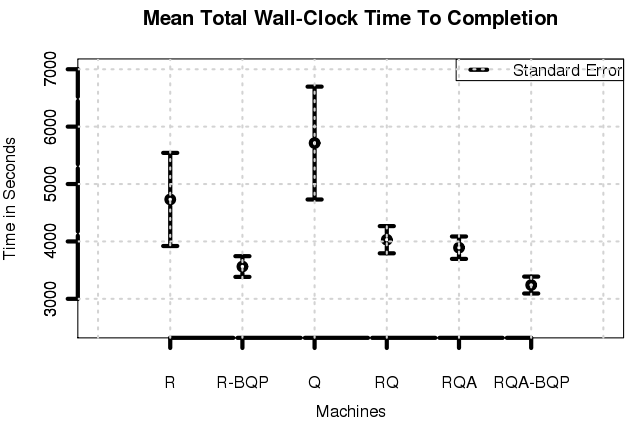
\includegraphics[scale=0.4]{Figure7.png}}
\subfigure{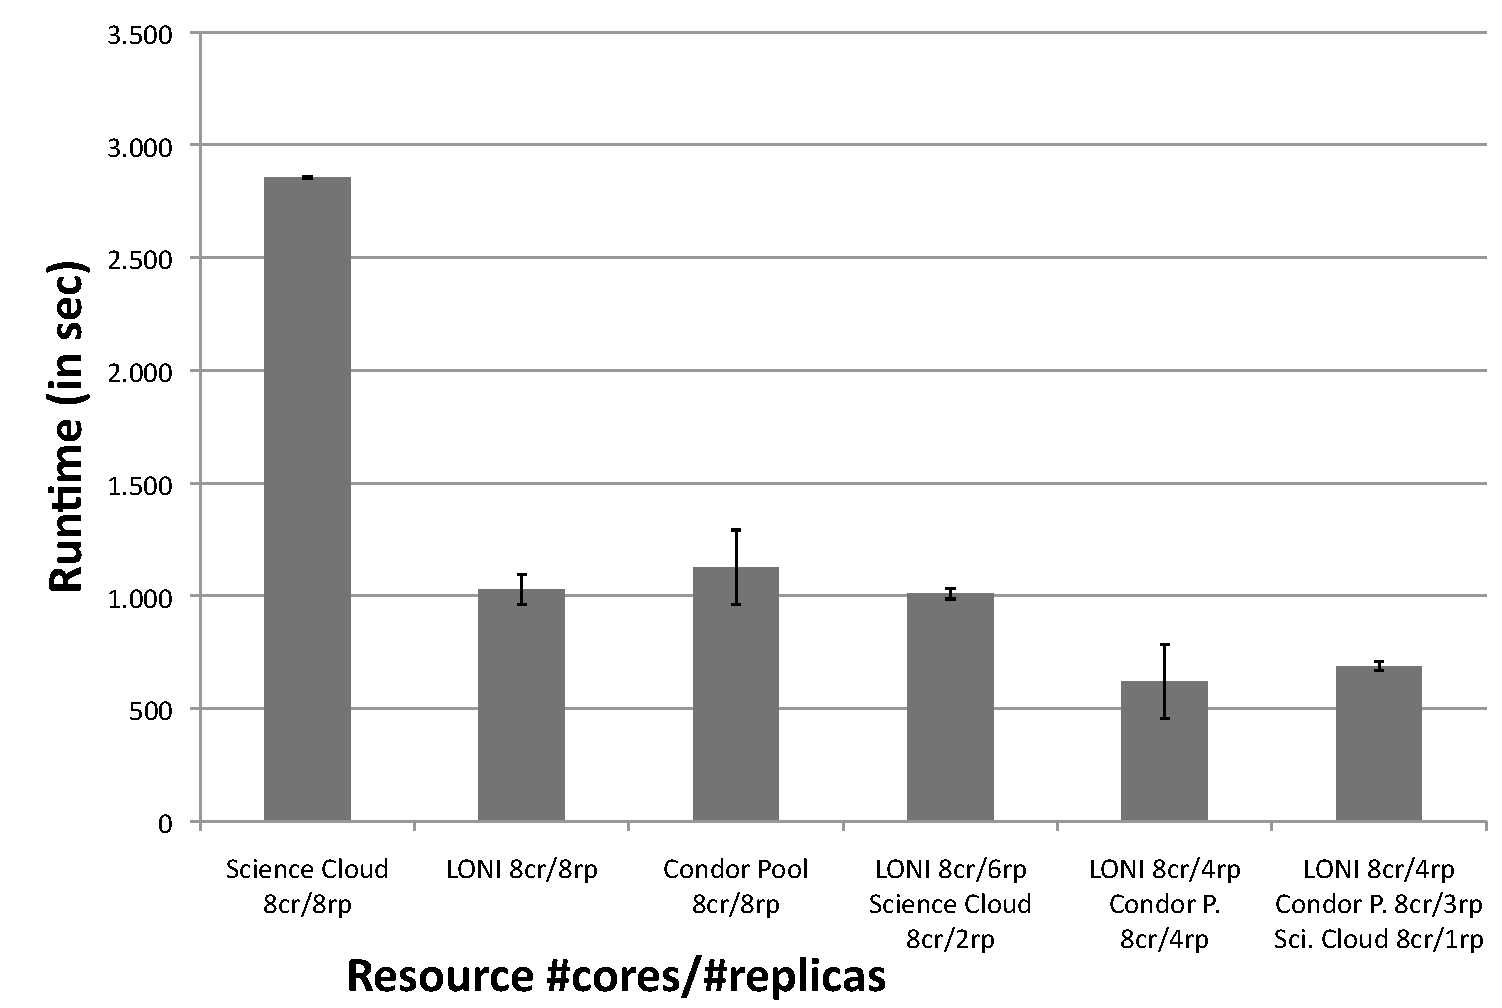
\includegraphics[scale=0.25]{8replica_scenario_grid_condor_cloud.pdf}}
\end{center}
\caption{\small Demonstrating the effectiveness of Distributed Applications Developed  Using SAGA to Scale-Out over multiple resources {\it concurrently}. From Left to Right, Performance as measured by the time-to-completeness of a well-defined workload when using: (i) Ranger only (ii) Ranger (with BQP service) only, (iii) QueenBee only, (iii) Ranger and QueenBee, (iv) Ranger, QueenBee and Abe concurrently (v) Ranger, QueenBee and Abe when using BQP service. From Ref.~\cite{gmac} and ~\cite{saga-ccgrid10}}
\label{fig:results}
\end{figure}

% \begin{figure} \begin{center} 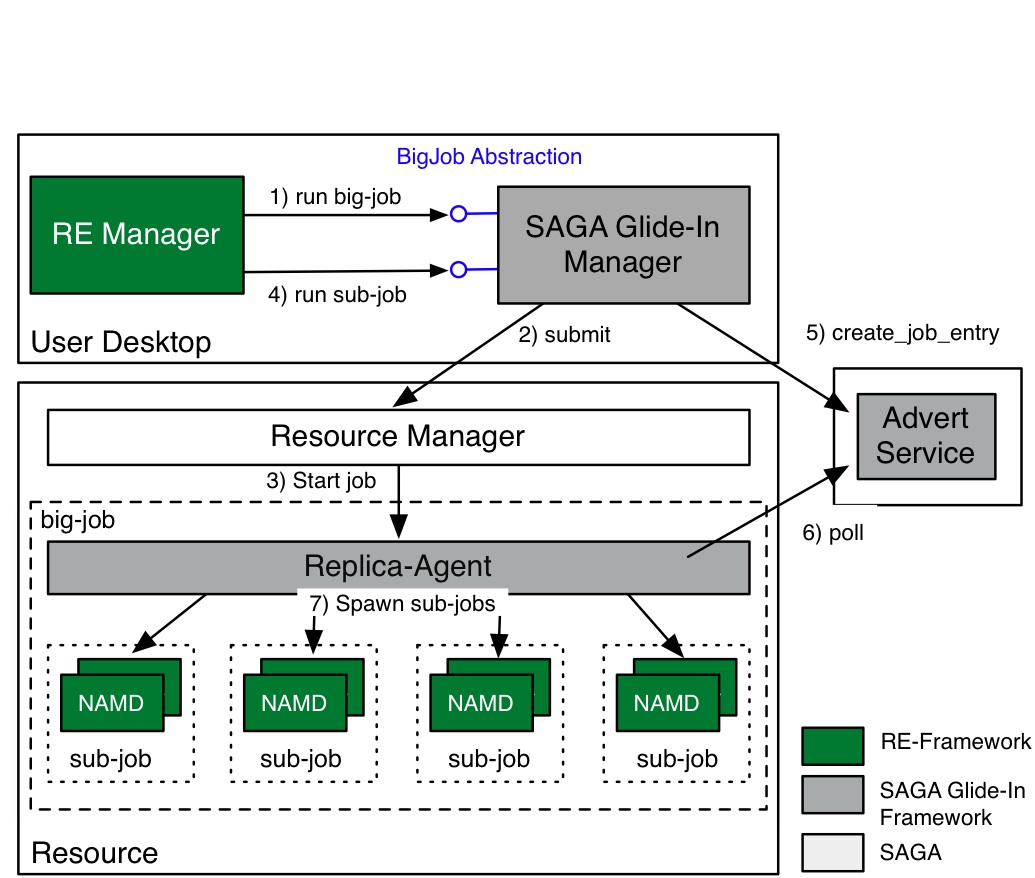
\includegraphics[scale=0.55]{DARE-MD} \end{center} \caption{Schematic of Distributed Adaptive Replica Exchange framework using the BigJob abstraction that is built upon SAGA. It is proposed that DARE-MD framework will ultimately become part of the GridChem Science Gateway (in which the PI and co-PI Kim are involved).} \label{fig:results} \end{figure}

\subsection*{Project 5b: CyberInfrastructure for CO$_2$ Sequestration Studies using SAGA: Autonomic Frameworks}

Global energy needs today present serious challenges: the increasing demand for energy must be met, 
however at the same time the emissions of greenhouse gases into the atmosphere must be reduced. 
Even as alternative energy sources continue to develop and gain popularity, the fact remains that 
fossil carbon resources will continue to be in heavy use (in both developing and industrialized 
countries) and consequently generate large volumes of carbon dioxide ~\cite{GeoRPT,Pawar}. The 
atmospheric impact of this greenhouse gas can be abated through capturing and sequestering 
significant fractions of the produced CO$_2$.

For long-term storage of large volumes of CO$_2$, porous subsurface geologic formations are ideal 
candidates: these are the same formations responsible for the existence of oil and gas reservoirs. 
Indeed much the technology behind carbon dioxide sequestration (including drilling, gas injection, 
reservoir management and of course reservoir simulation) stems from drilling, petroleum and 
reservoir engineering. Injecting CO$_2$ into an oil-gas reservoir can also lead to improved oil 
recovery by ``pushing out'' the oil and gas for production, this allows for reduced net cost 
through increased revenues from oil and gas production ~\cite{EORBook}.

% \begin{figure}
% \begin{center}
% 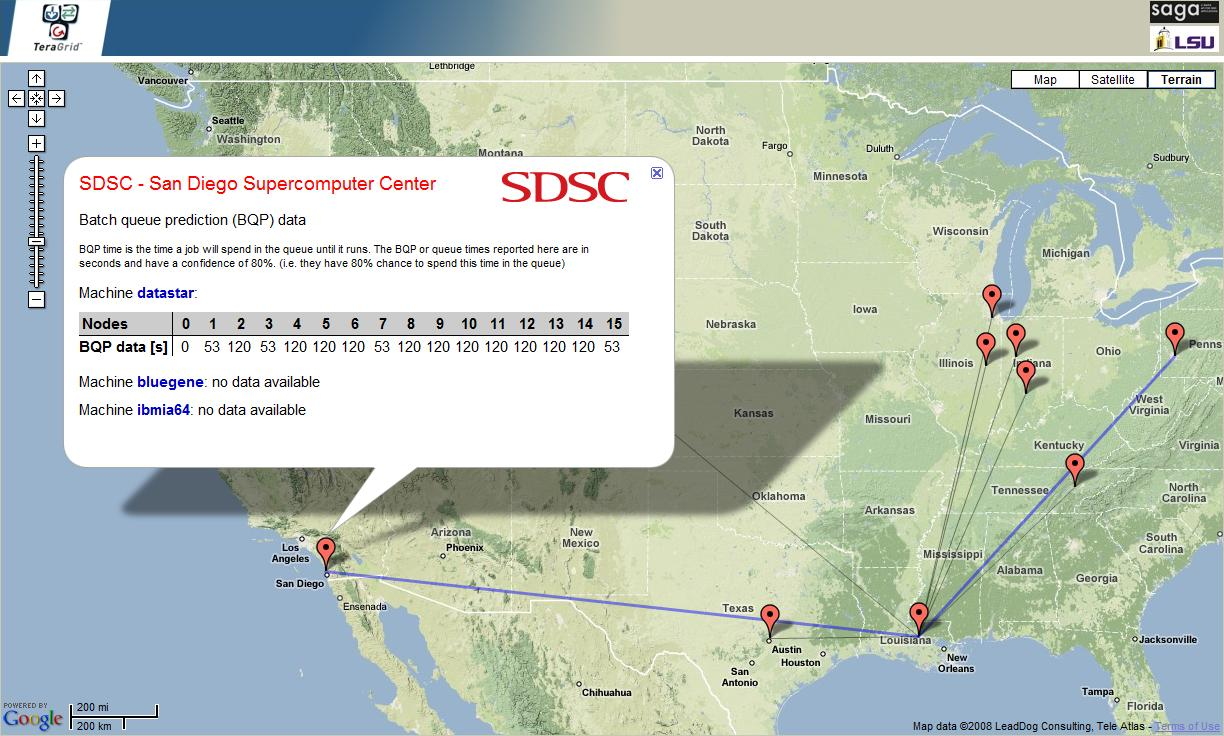
\includegraphics[scale=0.33]{gmaps_bqp.jpg}
% \end{center}
% \caption{A snapshot of an application using batch-queue-prediction system to dynamically determine the best resource to spawn a sub-task to; the noteworthy point is that the entire decision process is at the application level -- the fact that the application has to spawn a job of requirements X is mapped to a resource requirements, BQP is used to determine the resource based upon optimal availability and then the application uses SAGA to spawn and launch the sub-task onto the chose resource. A paper demonstrating this feature working across the TeraGrid won the Performance Challenge Award at TeraGrid 2008 (Ref.~\cite{teragrid08})}
% \label{}
% \end{figure}

One of the major challenges in CO$_2$ sequestration is the characterization of reservoirs that are 
safe and secure, environmentally and geologically and are therefore promising candidates for CO$_2$ 
sequestration ~\cite{GeoRPT,Luigi,Pruess2004,Pawar}. To that end, some of our efforts are directed towards 
developing CyberInfrastructure tools, technologies and abstractions that facilitate large scale 
reservoir characterization and forecasting studies~\cite{gmac,Elkhamra2009,MSEScience,TG10yye00}.

Since the amount of information obtained directly from reservoirs is very small compared to the 
actual size of the reservoir, history matching techniques have been developed to match actual 
reservoir production with simulated reservoir production, therefore obtaining a more 
``satisfactory'' set of reservoir models. A promising approache to history matching is 
the use of Ensemble Kalman filters (EnKF) ~\cite{KalmanPaper, DO2007, LiEnKF07, DO2006,Burger98}
and their various extensions.

Of particular interest are the EnKF extensions that can handle multiple physical phenomena,
such as the geochemical interaction between CO$_2$, geologic formation and formation fluids.
These phenomena are important because they allow a deeper understanding
of the long term environmental effects of CO$_2$ sequestration. To perform the analysis
step of highly nonlinear, multi-physics simulations, more than one ensemble is used 
\cite{Zhang,White1987,Durlofsky1992,Ballin1993,Gilks96,vanLeeuwen2003}.

Models with different physics can be combined, either hierarchically or by pooling 
groups of models in computation of relevant gains. That is, different  columns (corresponding to  
vectors of sensitivities of a model parameter to all observation misfits) can be based on different 
ensembles. Consistency is preserved if the gain columns are applied to models or sub-ensembles,
if and only if the models and sub-ensembles were used in the gain calculation. Alternatively, one 
can ``cross''  the sub-ensembles gains \cite{Mitchell02,Anderson2007,Michalak2003}

Having multiple ensembles (co-ensembles or hierarchical ensembles) will naturally increase the
amount of SUs required. A single simulation spanning a 1 million grid cell domain and simulating
15 years of production, 15 years of production forecast and 15 years of CO$_2$ sequestration will
require approximately $445$ SUs on Ranger and $395$ on Kraken. A two ensemble study, each with 100 ensemble members, 
will therefore require $89,000$ SUs on Ranger and $79,000$ SUs on Kraken. We estimate we will run 
at least $6$ full production 
simulations: $3$ on Ranger ($267,000$ SUs)  and $3$ on Kraken ($237,000$). Running
full production studies as opposed to smaller test-cases is necessary for scientific insight as 
well as to ensure the scalability of 
the framework and its ability to handle real world CO$_2$ sequestration studies. Additionally, we 
will need to run several dozen smaller simulations for testing, calibration and development on 
Ranger as it is a machine we are very familiar with. Therefore we would like to request $40000$ SUs 
on Ranger and $250,000$ SUs on Kraken.

We would also like to request $50,000$ additional SUs on Ranger to continue to pursue our 
experimental autonomic, on-demand scientific computing research with hybrid Grid-Cloud systems. 
Ranger has been
used effectively for this purpose \cite{Cloud1,Cloud2}. Furthermore, we would like to
continue to develop our distributed computing infrastructure across TeraGrid resources,
and therefore request a $50,000$ SUs allocation across Abe, QueenBee and Lonestar for autonomic 
Grid technology development and testing.


% Ensemble Kalman filters are recursive filters that can be used to handle large, noisy data; the 
% data in this case would be the results and parameters from ensembles of reservoir models that are 
% sent through the filter to obtain the ``true state'' of the data. Since the reservoir model varies 
% from one ensemble to another, the run-time characteristics of the ensemble simulation are irregular 
% and hard to predict. Furthermore, at simulation times when real historical data is available, all 
% the data from the different ensembles at that simulation time must be compared to the actual 
% production data, before the simulations are allowed to proceed. This translates into a global 
% synchronization point for all ensemble members; hence performing large scale studies for complex 
% reservoirs in a reasonable amount of time would benefit greatly from the use of distributed, high 
% performance, high throughput and on-demand computing resources.




\begin{table}[!h]
\begin{center}
 \caption{Summary of allocation usage for a full CO$_2$ sequestration study of a depleted resevoir}
\begin{tabular}{| c | c | c|}
\hline
& On Ranger & On Kraken \\
\hline
SU cost per simulation for history matching& 445 SUs & 395 SUs\\
\hline
Typical number of cores per simulation & 128 & 128 \\
\hline
Typical duration with the above number of cores & 3:30 hours & 3:00 hours \\
\hline
Number of members per ensemble & 100 members & 100 members \\ 
\hline
Number of sub/co ensembles & 2 ensembles & 2 ensembles \\ 
\hline
Total number of simulations & 200 simulations & 200 simulations\\
\hline
Total SUs consumed for full studies & 89,000 SUs & 79,000 SUs\\
\hline
Total SUs consumed for $3$ full studies & 267,000 SUs & 237,000 SUs\\
\hline
Total SUs requested & 400,000 SUs & 250,000 SUs\\
\hline
\end{tabular}
\end{center}
\end{table}



% \begin{figure}
% \begin{center}
% \includegraphics*[scale=0.4,angle=0]{3StageKalmanFilter}
% \end{center}
% \caption{Schematic illustrating the variability between stages of a typical
%   ensemble Kalman filter based simulation. The end-to-end
%   application consists of several stages; in general at each stage the
%   number of models generated varies in size and duration. From References~\cite{teragrid08, gmac}}
% \label{fig:irregular_execution}
% \end{figure}



\subsection*{Project 5c: Utilizing Application-level Interoperability across TeraGrid and DEISA}

As part of NSF funded HPCOPS Award (till July 2011), we are leading a project to utilize the aggregated computational power of the Federated Grids of DEISA and TeraGrid. The aim of the project is to (i) work towards an integrated infrastructure that supports application level-interoperability and, (ii) having created the infrastructure, apply it to the dual challenge of understanding the conformational changes and determining the free energy of biological systems. Specifically, the high-level aim of this project is to enable scientific applications to utilise the federated capabilities of the TeraGrid, DEISA and LONI systems, to enhance the understanding of HIV-1 enzymes and epidermal growth factor receptors (EGFR) implicated in lung cancer -- important science drivers which form the basis of Project 3. The Computer Science aims of this project are to use several Replica-based and Replica-Exchange simulations for HIV-1 \& EGFR research, on multiple TeraGrid, LONI and DEISA resources, working concurrently towards the solution of a single problem instance -- the rapid computation of free-energies of binding with high-levels precision.

{\it Resource Requirements:} For Project 5c, we require 250,000 SUs. This is a somewhat experimental component of this proposal, where we do not have clear estimates and benchmarking data. However, based upon our experience/publications alluded to in the previous paragraph, each "experiment" that we conduct, (i.e. application that we develop), requires a minimum of 50,000 SUs. The TeraGrid-DEISA Interoperability project -- built upon validated and ready to run models, has already acquired significant resources (several million CPU hours) on DEISA machines; our request for 250K is to support initial production runs of the VPH (Virtual Physiological Human) models and test the infrastructure for Scale-Out tests -- intra-TeraGrid as well as TeraGrid-DEISA Grids, performed on the VPH Models.
 
% For example, running a reservoir simulation for a simulation time of two weeks (typical period of historical production data gathering) consumes roughly ten minutes on four cores.  With two hundred ensembles (typical number of ensembles), running for a simulation time of fifteen years will consume 48k SUs. This obviously is the medium range of simulations; a more detailed reservoir model will naturally consume more SUs per simulation, multiplied by a large number of ensembles and the SUs required to perform the history matching increases dramatically. To complete the forecast stage, we will need to run the same ensembles for an extended period of time (reservoir depletion/workover, enhanced oil recovery and CO$_2$ sequestration) which roughly would range between twenty to thirty years in simulation time, that is an additional 64k-96k SUs, placing the total in the range of 112k-144k SUs for a single complete reservoir study.


% \subsection{Associated Technical Developments, Collaborations \& Other High
% Performance Computing Resources}

% We plan to release the next version of our grid middleware Application Hosting Environment (AHE) in the second half of 2010 \cite{zasada2009,coveney2007}, during the proposed TRAC allocation.  The AHE provides simple graphical and command line interfaces to run applications on resources provided by grid computing infrastructures in addition to local campus-based clusters, while hiding from the user details of the underlying middleware in use by the distinct resource providers.  We are engaged in integrating AHE with a metascheduling framework, based on a computational mechanism design, which is mediated by software agents, to efficiently allocate work between a set of resources based on cost minimization and run time optimization.  The patient-specific clinical simulation work proposed in this TRAC will be supported by our plans to integrate support for SPRUCE (a system developed at Argonne National Labs for urgent computing by allowing users to run emergency jobs) within the AHE client interface, so that jobs submitted with SPRUCE tokens use the mechanisms provided by SPRUCE to preempt the current workload on a machine.


% We also plan to introduce a mechanism to host workflows in the AHE as virtualized applications, composed by orchestrating the execution of other AHE hosted applications. The purpose of workflow management systems is to automate common time consuming tasks that the scientist carries out when performing \emph{in silico} studies. With the planned developments, we can interact with workflows involving simulation pre-processing, launch and post-processing via the AHE in the same way as with a single application. This work is being done in collaboration with developers of the GSEngine workflow management tool within the European Union's (EU) Virtual Physiological Human (VPH) project.


% Use of the AHE and software from the SAGA project has allowed our research team to inter-operate between high performance computing resources in the US, UK and the EU.  Additionally, within our grid middleware development activities, we are working on a new mechanism, termed as Audited Credential Delegation, to allow controlled access to a single grid certificate for a group of users, authenticated by their local institutional security credentials, facilitated by AHE. This approach is being developed to address issues related to the scalability of the current X.509 certificate-based authentication model, which relies on each individual user obtaining and managing his/her own grid certificates. This project is being funded by the UK EPSRC grant (EP/D051754/1) entitled ``User-Friendly Authentication and Authorisation for Grid Environments''.


\section*{Supporting Grants}
%\jhanote{Shantenu to update. (i) ExTECNI, (ii) BIPAS and others.} 
%\subsection{Peer Reviewed Research:} 

The PI's research is supported by current NIH and NSF awards.  See PI's vitae for full grant listing.
The PI leads Work Package 4 of the NSF Funded Cybertools Project (http://www.cybertools.org) (NSF Award NSF/LEQSF(2007-10)-CyberRII-01; Total Value \$12M) and the \$15M NIH award supporting the Louisiana Biomedical Research Network (LBRN). Project 1 is partially supported by the Biosensors work activity of WP-1 of Cybertools.

Project 2 is funded by multiple awards, including a \$15M NIH Louisiana Biomedical Research Network Award (of which Jha is the co-PI and Director of the Bioinformatics and Computational Biology Core; award number 2 P20 RR016456-09), Louisiana Board of Regents award and an LSU Faculty Award (PI Jha). Project 2 has been supported by a LSU Faculty Research Award to PI Jha, in conjunction with multiple awards to Fareed Aboul-ela (Experimental Collaborator). Project 2 has also benefitted from a LONI Distinguished Graduate Assistantship to Wei Huang (PhD Student co-supervised by PI Jha and experimental collaborator Aboul-ela) Project 2 forms the basis for a large NSF proposal under review, {\it IIS 1029810 Macromolecular Choreography: Computational methods to detect conserved dynamic properties in non-coding RNAs}.

Project 3 is led by co-PI Coveney, who is the Principal Investigator of the \$12M EU FP7 Virtual Physiological Human Network of Excellence. Project 1 \& 4 are also supported by RealityGrid grant GR/R67699 funded by EPSRC (the UK equivalent of NSF). Coveney and Jha have active collaboration over eight years in the field of molecular dynamics, high performance, distributed \& grid computing and have co-authored 12 papers in these areas, and are currently writing several papers related to Project 1, 3 and 5c.
 
PI-Jha is the co-PI of LSU's HPCOPS NSF-OCI 0710874 award which also supports a large fraction of Projects 5a and 5c. Integration of SAGA with applications is part of Cybertools and the PI also holds multiple peer-reviewed awards for the development and integration of SAGA.  The Interoperability Project~\cite{interop_url} is currently funded by an NSF HPCOPS award, and is being executed by the PI (Jha).

In addition, the PI is the LSU-lead in the \$2M ExTENCI (OCI-1007115) project that aims to further interoperability between TeraGrid and Open Science Grid.  Project 5b is supported by NSF OCI award - ExTENCI: Extending Science Through Enhanced National Cyberinfrastructure (total \$2M, LSU share \$0.2M; Project Officer Barry Schneider).  Project 5b is also supported by UCoMS project, Department of Energy and Louisiana Board of Regents award No. DE-FG02- 04ER46136 (PI Chris White, LSU -- collaborator of PI Jha and co-PI el-Khamra); it also forms the basis of OIA 1028948 Cyber Enabled Geomodel Inversion (under review at NSF).

\subsection{Completmentary Computing Allocations:} In addition to the requested TeraGrid allocation, we currently have an allocation of 4.04 million Allocation Units (AUs) on the UK's Cray XT4 supercomputing resource associated with the EPSRC grant (EP/F00521/1) entitled ``Large scale lattice-Boltzmann simulation of liquid crystals'' for materials science research. Within the EU VPH Virtual Community project, we annually receive an allocation of 2.0M CPU hours on the EU's DEISA grid for our work in the bio-medical sciences domain.  (This computational allocation has been awarded to Coveney (PI); award number EU FP7-ICT-2007-5.3 223920 funded by the European Union with a start date of 06/01/2008 and expiration date of 11/30/2012).  We have been successful in the DEISA Extreme Computing Initiative (DECI) calls successively for the past several years, most recently gaining 700,000 CPU hours for our computational science activities.  (The most recent DECI computational allocation was awarded to Coveney (PI); award number EU RI-222919 funded by the European Union with a start date of 01/01/2009 and expiration date of 01/31/2010).

% \section{Senior Personnel}
% 
\textbf{Professor P.V. Coveney} holds a Chair in Physical Chemistry and is Director of the Centre for Computational Science (CCS) within the Department of Chemistry at UCL. He is an Adjunct Professor at Yale University, USA. He holds an Honorary Professorship in Computer Science, also at UCL. He is the Principal Investigator of the \$12M EU FP7 Virtual Physiological Human Network of Excellence. He led the UK/US TeraGyroid (RealityGrid grant GR/R67699) and SPICE (NSF Grant Numbers CA SCI-0525308 and CSA SCI-0438712 and EPSRC Grant EP/D500028/1) projects funded by EPSRC and NSF, and is the recipient of an HPC Challenge Award at Supercomputing 2003, an International Supercomputing Conference Award in 2004, an inaugral HPC Analytics Challenge Award at Supercomputing 2005 and an International Supercomputing Conference Life Sciences Award 2006. He is the recipient of a Transformational Science Challenge award as well as a recipient of two TeraGrid 5K Club awards for the codes HYPO4D and LB3D at TeraGrid'08. Professor Coveney is currently Chairman of the UK Collaborative Computational Projects (CCP) Steering Panel. He is the editor of the first single volume publication on scientific grid computing, published by \emph{Philosophical Transactions of the Royal Society A} (2005). He is a founding editor (with Peter Sloot and Jack Dongarra) of the Elsevier \emph{Journal of Computational Science} which will appear for the first time in 2010. Coveney and Jha have collaborated over seven years in the field of molecular dynamics, high performance, distributed \& grid computing and have co-authored 12 papers in these areas.

% \textbf{Dr Andrew Sherman} Dr. Sherman provides HPC support via the Yale Provost's Office for faculty and students, and is himself an expert on linear algebra methods in high performance computing.

% The present TeraGrid TRAC
% proposal contains two areas in which we will be collaborating with
% colleagues at Yale. These include biomedical research areas concerned
% with neurovascular modelling and stimulation, using HemeLB and patient
% specific HIV therapy based on rapid and accurate determination of
% protease-inhibitor binding affinities; and also in the determination
% of unstable periodic orbits based on the HYPO4D package. In both these
% areas, Dr. Sherman will lead and co-ordinate the participation of
% other Yale colleagues. He will contribute to our effort to improve the
% pre-conditioning of the variational relaxation procedure in order to
% enhance numerical convergence on candidate UPOs.  On 8 October 2009,
% the Presidents of Yale \& UCL signed a five-year collaboration
% agreement designed to provide for a deepening alliance§ between the
% two universities. In its initial phases, currently underway, this will
% focus on advancing biomedical research and healthcare on a global
% scale, through joint scientific research, clinical and educational
% effort. As the alliance widens, it is anticipated that more academic
% areas will become part of this formal agreement.

% One central area of immediate and longer term concern is sharing of
% computational resources and facilities. The UCL-Yale consortium aims
% to conduct international science through sharing of resources on both
% sides of the Atlantic. The current proposal will help us to build
% joint computational effort in relevant research areas, with reciprocal
% resources being made available in UK and EU via DEISA and related
% resources. In addition, as part of their alliance, Yale and UCL are
% exploring ways to link each others' sites via an international high
% speed network.

% \begin{comment}
% Yale \& UCL are planning to link each others' sites via an
% international high speed network in 2010, funding for which will come
% from the two institutions, UK Government and EU (as part of the ELIXIR
% project which will develop sustainable data infrastructures across
% Europe). JA.NET (the UK's education and research network,
% http://www.ja.net) will provide the 10Gb/s dedicated connectivity via
% their LightPath (http://www.ja.net/services/lightpath) link
% procurements to DANTE (DANTE Delivery of Advanced Network Technology
% to Europe; http://www.dante.net), crossing under the Atlantic to
% Internet2 and hence on to Yale \& TeraGrid.
% \end{comment}

% \subsection{Associated Technical Developments, Collaborations \& Other High
% Performance Computing Resources}

% We plan to release the next version of our grid middleware Application Hosting Environment (AHE) in the second half of 2010 \cite{zasada2009,coveney2007}, during the proposed TRAC allocation.  The AHE provides simple graphical and command line interfaces to run applications on resources provided by grid computing infrastructures in addition to local campus-based clusters, while hiding from the user details of the underlying middleware in use by the distinct resource providers.  We are engaged in integrating AHE with a metascheduling framework, based on a computational mechanism design, which is mediated by software agents, to efficiently allocate work between a set of resources based on cost minimization and run time optimization.  The patient-specific clinical simulation work proposed in this TRAC will be supported by our plans to integrate support for SPRUCE (a system developed at Argonne National Labs for urgent computing by allowing users to run emergency jobs) within the AHE client interface, so that jobs submitted with SPRUCE tokens use the mechanisms provided by SPRUCE to preempt the current workload on a machine. We also plan to introduce a mechanism to host workflows in the AHE as virtualized applications, composed by orchestrating the execution of other AHE hosted applications. The purpose of workflow management systems is to automate common time consuming tasks that the scientist carries out when performing \emph{in silico} studies. With the planned developments, we can interact with workflows involving simulation pre-processing, launch and post-processing via the AHE in the same way as with a single application. This work is being done in collaboration with developers of the GSEngine workflow management tool within the European Union's (EU) Virtual Physiological Human (VPH) project.

% In addition to the requested TeraGrid allocation, we currently have an allocation of 4.04 million Allocation Units (AUs) on the UK's Cray XT4 supercomputing resource associated with the EPSRC grant (EP/F00521/1) entitled ``Large scale lattice-Boltzmann simulation of liquid crystals'' for materials science research. Within the EU VPH Virtual Community project, we annually receive an allocation of 2.0M CPU hours on the EU's DEISA grid for our work in the bio-medical sciences domain.  (This computational allocation has been awarded to Coveney (PI); award number EU FP7-ICT-2007-5.3 223920 funded by the European Union with a start date of 06/01/2008 and expiration date of 11/30/2012).  We have been successful in the DEISA Extreme Computing Initiative (DECI) calls successively for the past several years, most recently gaining 700,000 CPU hours for our computational science activities.  (The most recent DECI computational allocation was awarded to Coveney (PI); award number EU RI-222919 funded by the European Union with a start date of 01/01/2009 and expiration date of 01/31/2010).  Use of the AHE and software from the SAGA project has allowed our research team to inter-operate between high performance computing resources in the US, UK and the EU.  Additionally, within our grid middleware development activities, we are working on a new mechanism, termed as Audited Credential Delegation, to allow controlled access to a single grid certificate for a group of users, authenticated by their local institutional security credentials, facilitated by AHE. This approach is being developed to address issues related to the scalability of the current X.509 certificate-based authentication model, which relies on each individual user obtaining and managing his/her own grid certificates. This project is being funded by the UK EPSRC grant (EP/D051754/1) entitled ``User-Friendly Authentication and Authorisation for Grid Environments''.

\begin{comment}	
\emph{We need to ensure we address point raised last time, by citing 
reciprocal activities in UK/EU, and equivalnet utilization of DEISA REOSOURCEes.}
We have an allocation of X million AUs on UK's Cray XT4 supercomputer associated
with the UK EPSRC Grant(LSLBLC NO.) which
will support the projects within the bio-materials science domain. We plan
to perform complementary activities on EU's DEISA grid 
in the biomedicine domain, where the work is
supported by EU FP6 and FP7 funding and the new UCL-Yale initiative. 
We have been successful in the DEISA Extreme Computing Initiative (DECI)
calls successively for the past two years in gaining access to some of the
biggest supercomputers in the EU. Use of SAGA and AHE 3.0 will allow us to
seamlessly inter-operate between high performance computing resources in the
US and EU.
\end{comment} 
%dan katz cyber infrastructure. \newline\newline
%transatlantic lightpaths bbrsc nih \newline\newline
%ucl-yale initiative  


% Part of EnKF work is funded by the UCoMS project, Department of Energy and Louisiana
% Board of Regents award No. DE-FG02- 04ER46136


\section*{Summary}
% In summary, our request is for 1.25M SUs bound (non-roaming) to Ranger, 0.75M SUs bound to Kraken and a 750K roaming allocation over QB-ABE/Ranger/Kraken.  To state the obvious, if a primary aim of our work is to investigate the ability of distributed applications to {\it Scale-Out}, then it is imperative that there be an underlying resource allocation to support the work. We aim to develop frameworks such as Lazarus and Faust to support the ability of applications to {\it Scale-Out} in a manner that is independent of the specifics of the applications.  By extension, in order to scale-out to the TeraGrid and DEISA combined resources (one of the motivations for interoperability), we will also have to scale-out on the TeraGrid.  In general, there are instances where we have chosen to request non-roaming allocations but request more than one machine for the same project; this is to hedge against lengthy, but more challengingly, variable queue length (load) factors. However, the bulk of our resource request is non-roaming ($\approx$ 75\%).

\begin{table}[!h]
\begin{center}
  \caption{Resource distribution requests for different projects \jhanote{This will need revision and updating} \newline}
\label{table:systems}
\begin{tabular}{|c| c | c | }
\hline 
Project & Resource & Total Request \\ 
\hline
1 & Ranger  & TBD \\
1 & Kraken &  TBD  \\
\hline
2 & Ranger & TBD \\
2 & Kraken & TBD \\
\hline
3a & Abe-QB/Kraken/Ranger & TBD \\
3b & Abe-QB/Kraken/Ranger & TBD \\
\hline
4a & Abe-QB/Kraken/Ranger & TBDK \\
\hline
5a & Abe-QB/Kraken/Ranger & TBD \\
5b & Abe-QB/Kraken/Ranger & TBD \\
\hline
\end{tabular}
\end{center}
\end{table}


\bibliographystyle{unsrt}


%\begin{thebibliography}{10}

\bibitem{jarz}
C. Jarzynski. Phys. Rev. Lett., 78(14):2690�2693, 1997.

\bibitem{namd}
J. Philips et al. Journal of Computational Chemistry. 26, 1781-1802, 2005.

\bibitem{akeson}
M. Akeson et al. Biophys. J., 77(6):3227�3233, 1999.

\bibitem{foloppe}
N. Foloppe et al. Drug Discovery Today. 11, 1019-1027, 2006.

\bibitem{mandal}
M. Mandal et al. Nat Rev Mol Cell Biol. 5(6), 451-63, 2004.

\bibitem{brooke}
B. A. M. McDaniel et al. Proc. Natl. Acad. Sci. U.S.A. 100, 3083-3088, 2003.

\bibitem{SAM-I-NAR2009}
W.~Huang, J.~Kim, S.~Jha, and F.~Aboul-ela.
\newblock A mechanism for s-adenosyl methionine assisted formation of a
  riboswitch conformation: A small molecule with a strong arm.
\newblock {\em Nucleic Acid Research}, submitted.

\bibitem{montange}
R. K. Montange et al. Nature. 255, 1172-1175, 2006.

\bibitem{alberto}
P. Alberto, et al. Biophysical Journal. 92, 3817-3829, 2007.

\bibitem{wang}
J. Wang et al. Journal of Molecular Graphics and Modelling , 25, 247260, 2006,.

\bibitem{moe}
Molecular Operating Environment (MOE 2007.9), Chemical Computing Group (CCG).

\bibitem{saga_url}
The Simple API for Grid Applications, http://saga.cct.lsu.edu.

\bibitem{saga_escience07}
S.~Jha, H.~Kaiser, Y.~El Khamra, and O.~Weidner.
\newblock Design and implementation of network performance aware applications
  using saga and cactus.
\newblock In {\em Accepted for 3rd IEEE Conference on eScience2007 and Grid
  Computing, Bangalore, India.}, 2007.

\bibitem{gmac}
Y.~El Khamra and S.~Jha.
\newblock Title: {Developing Autonomic Distributed Scientific Applications: A
  Case Study From History Matching Using Ensemble Kalman-Filters}.
\newblock In {\em Sixth International Conference on Autonomic Computing, 2009.
  ICAC '09 (Barcelona)}. IEEE, 2009.

\bibitem{REMD-PhilTranA2009}
A.~Luckow, S.~Jha, J.~Kim, A.~Merzky, and B.~Schnor.
\newblock Adaptive distributed replica-exchane simulations.
\newblock {\em Phil. Tran. A}, 367:2595, 2009.

\bibitem{saga_loosely_coupled}
Developing Scientific Applications With Loosely-Coupled Sub-Tasks, accepted
  International Conference on Computational Science (ICCS), in Baton Rouge, Jan
  2009.

\bibitem{teragrid08}
S.~Jha, K.~Hartmut, Y.~El Khamra, and O.~Weidner.
\newblock Developing adaptive scientific applications with hard to predict
  runtime resource requirements with saga.
\newblock In {\em Proceedings of the TeraGrid 2008 Conference}, 2008.

\bibitem{saga_data_intensive}
Programming Abstraction for Data Intensive Computing on Clouds and Grids,
  accepted at Intl. Workshop on Cloud Computing, 2009, in conjunction with
  CCGrid2009. Draft at:
  {\href{http://www.cct.lsu.edu/~sjha/publications/saga\_data\_intensive.pdf}{%
\url{http://www.cct.lsu.edu/~sjha/publications/saga\_data\_intensive.pdf}}}.

\bibitem{saga_grid_cloud}
Application Level Interoperability between Clouds and Grids accepted for First
  International Workshop on Grids and Clouds, held in conjunction with
  Conference on Grid and Pervasive Computing, Geneva, 2009. Draft at: \\
  \url{http://www.cct.lsu.edu/~sjha/publications/saga\_cloud\_interop.pdf}.

\bibitem{GeoRPT}
D.~J.~DePaolo et~al.
\newblock Basic research needs for geosciences:facilitating 21st century energy
  systems.
\newblock {\em Office of Basic Energy Sciences, U.S. Department of Energy},
  2007.

\bibitem{EORBook}
D.~W. Green and G.~P. Willhite.
\newblock {\em Enhanced Oil Recovery}, volume~6.
\newblock 1998.

\bibitem{Luigi}
L.~Marini.
\newblock {\em Geological Sequestration of Carbon Dioxide, Volume 11:
  Thermodynamics, Kinetics, and Reaction Path Modeling (Developments in
  Geochemistry)}, volume~11.
\newblock 2007.

\bibitem{KalmanPaper}
R.~E. Kalman.
\newblock A new approach to linear filtering and prediction problems.

\bibitem{DO2007}
Y.~Gu and D.~S. Oliver.
\newblock An iterative ensemble kalman filter for multiphase fluid flow data
  assimilation.
\newblock {\em SPE Journal}, 12(4):438--446, 2007.

\bibitem{LiEnKF07}
X.~Li, C.~White, Z.~Lei, and G.~Allen.
\newblock Reservoir model updating by ensemble kalman filter-practical
  approaches using grid computing technology.
\newblock In {\em Petroleum Geostatistics 2007}, Cascais,Portugal, August 2007.

\bibitem{DO2006}
Y.~Gu and D.~S. Oliver.
\newblock The ensemble kalman filter for continuous updating of reservoir
  simulation models.
\newblock {\em Journal of Engineering Resources Technology}, 128(1):79--87,
  2006.

\bibitem{interop_url}
TeraGrid-LONI Interoperabilty Project, {\it A Science-Driven Project Using
  Advanced CyberInfrastructure funded by NSF via a HPCOPS award to LONI},
  {\url{http://www.teragridforum.org/mediawiki/index.php?title=LONI-TeraGrid-D%
EISA\_Interoperabilty\_Project}}.

% \end{thebibliography}
% \begin{thebibliography}{10}

\bibitem{zasada2009}
P.~V. Coveney and S.~J. Zasada.
\newblock Virtualizing access to scientific applications with the {Application
  Hosting Environment}.
\newblock {\em Comp. Phys. Comm.}, 180(12):2513--2525, 2009.

\bibitem{coveney2007}
P.~V. Coveney, R.~S. Saksena, S.~J. Zasada, M.~McKeown, and S.~Pickles.
\newblock The application hosting environment: Lightweight middleware for
  grid-based computational science.
\newblock {\em Comp. Phys. Comm.}, 176:406--418, 2007.

\bibitem{chaos-book}
P.~Cvitanovi{\'{c}}, R.~Artuso, R.~Mainieri, G.~Tanner, G.~Vattay, N.~Whelan,
  and A.~Wirzba.
\newblock {\em Chaos: Classical and Quantum (http://www.chaosbook.org/)}.
\newblock Niels Bohr Institute, Copenhagen, 2005.

\bibitem{artuso}
R.~Artuso, E.~Aurell, and P.~Cvitanovi{\'{c}}.
\newblock Recycling of strange sets \uppercase{i}: cycle expansions.
\newblock {\em Nonlinearity}, 3:325--359, 1998.

\bibitem{bohr-jensen}
T.~Bohr, M.~H. Jensen, G.~Paladin, and A.~Vulpiani.
\newblock {\em Dynamical Systems Approach to Turbulence (Cambridge Nonlinear
  Science Series)}.
\newblock Cambridge University Press, 1998.

\bibitem{lan-cvitanovic}
Y.~Lan and P.~Cvitanovi\ifmmode~\acute{c}\else \'{c}\fi{}.
\newblock Variational method for finding periodic orbits in a general flow.
\newblock {\em Phys. Rev. E}, 69(1):016217, 2004.

\bibitem{Comput-HYPO4D}
L.~Fazendeiro, B.~M. Boghosian, P.~V. Coveney, and J.~L{\"{a}}tt.
\newblock Unstable periodic orbits in turbulent hydrodynamics.
\newblock {\em Submitted to the Journal of Computational Science}, 2009.

\bibitem{draft-bogh-tam2}
B.~M. Boghosian, P.~V. Coveney, L.~Fazendeiro, J.~L{\"{a}}tt, J.~Tam, and
  H.~Tang.
\newblock A computational program for the dynamical systems approach to
  turbulence.
\newblock {\em Submitted to Journal of Computational Science}, 2010.

\bibitem{saksenapetascale}
R.~S. Saksena, B.~M. Boghosian, L.~Fazendeiro, O.~A. Kenway, S.~Manos,
  M.~Mazzeo, S.~K. Sadiq, J.~L. Suter, D.~Wright, and P.~V. Coveney.
\newblock Real science at the petascale.
\newblock {\em Phil. Trans. R. Soc. A}, 367(1897):2557--2571, 2009.

\bibitem{viswanath2007}
D.~Viswanath.
\newblock Recurrent motions within plane {Couette} turbulence.
\newblock {\em J. Fluid Mech.}, 580:339--358, 2007.

\bibitem{gibson2008}
J.~F. Gibson, J.~Halcrow, and P.~Cvitanovi\'{c}.
\newblock Visualizing the geometry of state space in plane couette flow.
\newblock {\em J. Fluid Mech.}, 611:107--130, 2008.

\bibitem{dennis1996}
J.~E. Dennis~Jr and R.~B. Schnabel.
\newblock Numerical methods for unconstrained optimization and nonlinear
  equations.
\newblock {\em SIAM}, 1996.

\bibitem{doctors2009}
G.~M. Doctors, M.~D. Mazzeo, and P.~V. Coveney.
\newblock {A computationally efficient method for simulatioon of fluid flow in
  elastic pipes in toand three dimensions}.
\newblock {\em Submitted to Computer Physics Communications}, 2009.

\bibitem{mazzeo2010}
M.~D. Mazzeo, S.~Manos, and P.~V. Coveney.
\newblock {In situ ray tracing and computational steering for interactive blood
  flow simulation}.
\newblock {\em Computer Physics Communications}, 181:355--370, 2010.

\bibitem{manostg08}
S.~Manos, S.~Zasada, M.~D. Mazzeo, R.~Haines, G.~Doctors, S.~Brew, R.~Pinning,
  J.~Brooke, and P.~V. Coveney.
\newblock {Patient specific whole cerebral blood flow simulation: A future role
  in surgical treatment for neurovascular pathologies}.
\newblock {\em Winner of 'Transformational Science Challenge' award at TeraGrid
  2008}, 2008.

\bibitem{manoshpdc08}
S.~Manos, M.~Mazzeo, O.~Kenway, P.~V. Coveney, N.~T. Karonis, and B.~Toonen.
\newblock Distributed {MPI} cross-site run performance using mpig.
\newblock In {\em HPDC '08: Proceedings of the 17th international symposium on
  High performance distributed computing}, pages 229--230, New York, NY, USA,
  2008. ACM.

\bibitem{manosctw08}
S.~Manos, S.~Zasada, and P.~V. Coveney.
\newblock {Life or Death Decision-making: The Medical Case for Large-scale,
  On-demand Grid Computing}.
\newblock {\em CTWatch Quarterly}, 4(1), 2008.

\bibitem{mazzeo2008}
M.~D. Mazzeo and P.~V. Coveney.
\newblock {HemeLB: A high performance parallel lattice-Boltzmann code for large
  scale fluid flow in complex geometries}.
\newblock {\em Computer Physics Communications}, 178(12):894--914, 2008.

\bibitem{saksena2008}
R.~S. Saksena and P.~V. Coveney.
\newblock Self-assembly of ternary cubic, hexagonal, and lamellar mesophases
  using the lattice-{B}oltzmann kinetic method.
\newblock {\em J. Phys. Chem. B}, 112(10):2950 -- 2957, 2008.

\bibitem{harting2004_2}
J.~Harting, Chin. J., M.~Venturoli, and P.~V. Coveney.
\newblock Large-scale grid-enabled lattice-boltzmann simulations of complex
  fluid flow in porous media and under shear.
\newblock {\em Phil. Trans. R. Soc. Lond. A}, 362:1703--1722, 2004.
\newblock there is an updated publication from 2005.

\bibitem{cates2008sm}
M.~E. Cates and P.~S. Clegg.
\newblock Bijels: {A} new class of soft materials.
\newblock {\em Soft Matter}, 4:2132--2138, 2008.

\bibitem{saksena2009_2}
R.~S. Saksena and P.~V. Coveney.
\newblock Shear rheology of amphiphilic cubic liquid crystals from large-scale
  kinetic lattice-boltzmann simulations.
\newblock {\em Soft Matter}, 5:4446--4463, 2009.

\bibitem{saksena1024}
R.~S. Saksena and P.~V. Coveney.
\newblock Defect texture dynamics under couette flow in amphiphilic liquid
  crystals from large-scale lattice-boltzmann simulations. {Preprint} 2010.

\bibitem{saksena2009}
R.~S. Saksena and P.~V. Coveney.
\newblock Rheological response and dynamics of an amphiphilic diamond phase.
\newblock {\em Proc. R. Soc. A}, 465:1977--2002, 2009.

\bibitem{saksenaahm09}
R.~S. Saksena, S.~J. Zasada, M.~D. Mazzeo, and P.~V. Coveney.
\newblock Petascale lattice-{B}oltzmann simulations of amphiphilic cubic liquid
  crystals. {Preprint 2010.}

\bibitem{bmb2005}
B.~M. Boghosian and P.~V. Coveney.
\newblock Scientific applications of grid computing.
\newblock {\em Computing in Science and Engineering}, 7(5):10--13, 2005.

\bibitem{blake-coveney-clarke-pickles-05}
R.~J. Blake, P.~V. Coveney, P.~Clarke, and S.~M. Pickles.
\newblock {\em Scientific Programming}, 13:1--17, 2005.

\bibitem{mckeown_ptrsla05}
R.~Haines, M.~McKeown, S.~M. Pickles, R.~L. Pinning, A.~R. Porter, and
  M.~Riding.
\newblock The service architecture of the teragyrid experiment.
\newblock {\em Phil. Trans. R. Soc. A}, 363:1743--1755, 2005.

\bibitem{hector}
{h}ttp://www.hector.ac.uk.

\bibitem{jens}
Private Communication. {Also see
  {www.hc-europa.eu/files/registrationTAM/6-Florian\%20JANOSCHEK.pdf}}.

\bibitem{JPCC_2007}
J.~L.~Suter \emph{et al}.
\newblock Large-scale molecular dynamics study of montmorillonite clay:
  Emergence of undulatory fluctuations and determination of material
  properties.
\newblock {\em J. Phys. Chem. C}, 111(23):8248--8259, 2007.

\bibitem{Franchi}
M.~Franchi, J.~P. Ferris, and E.~Gallori.
\newblock Cations as mediators of the adsorption of nucleic acids on clay
  surfaces in prebiotic environments.
\newblock {\em {Origins of Life and Evolution of the Biosphere}}, {33}:{1--16},
  {2003}.

\bibitem{Huang}
W. H. Huang and J. P. Ferris.
\newblock One-step, regioselective synthesis of up to 50-mers of {RNA}
  oligomers by montmorillonite catalysis.
\newblock {\em {Journal of the American Chemical Society}}, {128}:{8914--8919},
  {2006}.

\bibitem{understanding}
B.~Chen, J.~R.~G. Evans, H.~C. Greenwell, P.~Boulet, P.~V. Coveney, A.~A.
  Bowden, and A.~Whiting.
\newblock A critical appraisal of polymer-clay nanocomposites.
\newblock {\em Chem. Soc. Rev.}, 37:568--594, 2007.

\bibitem{Thyveetil}
M.-A. Thyveetil, P.~V. Coveney, J.~L. Suter, and H.~C. Greenwell.
\newblock Emergence of undulations and determination of materials properties in
  large-scale molecular dynamics simulation of layered double hydroxides.
\newblock {\em Chem. Mater.}, 19(23):5510--5523, 2007.

\bibitem{Thyveetil_JACS}
M.-A. Thyveetil, P.V. Coveney, H.~C. Greenwell, and J.~L. Suter.
\newblock Computer simulation study of the structural stability and materials
  properties of {DNA}-intercalated layered double hydroxides.
\newblock {\em J. Am. Chem. Soc.}, 130(14):4742--4756, 2008.

\bibitem{Soft_Matter1}
J.~L. Suter and P.~V. Coveney.
\newblock Computer simulation study of the materials properties of intercalated
  and exfoliated poly(ethylene)glycol clay nanocomposites.
\newblock {\em Soft Matter}, 5:2239, 2009.

\bibitem{Soft_Matter2}
J.~L. Suter and P.~V. Coveney.
\newblock Materials properties of clay nanocomposites: onset of negative
  {Poisson} ratio in large-scale molecular dynamics simulation.
\newblock {\em Soft Matter}, 5:3896--3904, 2009.

\bibitem{LAMMPS}
S.~J. Plimpton.
\newblock Fast parallel algorithms for short-range molecular dynamics.
\newblock {\em J. Comp. Phys.}, 117:1--19, 1995.

\bibitem{LAMMPS_2005}
S.~Plimpton.
\newblock Large-scale atomic/molecular massively parallel simulator;
  http://www.cs.sandia.gov/$\sim$sjplimp/lammps.html.
\newblock Sandia National Laboratories, Albuquerque, 2005.

\bibitem{rRESPA}
M.~Tuckerman, B.~J. Berne, and G.~J. Martyna.
\newblock Reversible multiple time scale molecular dynamics.
\newblock {\em J. Chem. Phys.}, 97:1990--2001, 1992.

\bibitem{Hockney_book}
R.~W. Hockney and J.~Eastwood.
\newblock {\em Computer Simulation Using Particles}.
\newblock McGraw-Hill, New York, 1981.

\bibitem{Stoica2008}
I.~Stoica, S.K. Sadiq, and P.V. Coveney.
\newblock Rapid and accurate prediction of binding free energies for
  saquinavir-bound {HIV}-1 proteases.
\newblock {\em Journal of the American Chemical Society}, 130(8):2639--2648,
  2008.

\bibitem{Genheden2009}
S.~Genheden and U.~Ryde.
\newblock How to obtain statistically converged {MM/PBSA} results.
\newblock {\em Journal of Computational Chemistry}, 2009.
\newblock Published online in July 2009.

\bibitem{Sadiq2010}
S.K. Sadiq, D.W. Wright, O.A. Kenway, and P.V. Coveney.
\newblock {Accurate Ensemble Molecular Dynamics Binding Free Energy Ranking of
  Multi-Drug-Resistant HIV-1 Proteases}.
\newblock {\em Journal of Chemical Information and Modelling}, 50(5):890-–905, 2010.

\bibitem{Ohtaka2003}
H.~Ohtaka, A.~Schon, and E.~Freire.
\newblock Multidrug resistance to {HIV-1} protease inhibition requires
  cooperative coupling between distal mutations.
\newblock {\em Biochemistry}, 42(46):13659--13666, Nov 2003.

\bibitem{Ivetac2009}
A.~Ivetac and J.A. McCammon.
\newblock {Elucidating the inhibition mechanism of HIV-1 non-nucleoside reverse
  transcriptase inhibitors through multicopy molecular dynamics simulations.}
\newblock {\em J Mol Biol}, 388(3):644--658, May 2009.

\bibitem{Sadiq2008}
S.~K. Sadiq, M.~D. Mazzeo, S.~J. Zasada, S.~Manos, I.~Stoica, C.~V. Gale, S.~J.
  Watson, P.~Kellam, S.~Brew, and P.~V. Coveney.
\newblock Patient-specific simulation as a basis for clinical decision-making.
\newblock {\em Philosophical Transactions of the Royal Society A: Mathematical,
  Physical and Engineering Sciences}, 366:3199--3219, 2008.

\bibitem{Sadiq2008a}
S.~K. Sadiq, D.~W. Wright, S.~J. Watson, S.~J. Zasada, I.~Stoica, and P.~V.
  Coveney.
\newblock An automated molecular simulation-based binding affinity calculator
  for ligand-bound {HIV}-1 proteases.
\newblock {\em Journal of Chemical Information and Modeling}, 48:1909--1919,
  2008.

\bibitem{Hess2008}
B.~Hess, C.~Kutzner, D.~van~der Spoel, and E.~Lindahl.
\newblock Gromacs 4: Algorithms for highly efficient, load-balanced, and
  scalable molecular simulation.
\newblock {\em Journal of Chemical Theory and Computation}, 4:435--447, 2008.

\bibitem{Phillips2005}
J.~C. Phillips, R.~Braun, W.~Wang, J.~Gumbart, E.~Tajkhorshid, E.~Villa,
  C.~Chipot, R.~D. Skeel, L.~Kale, and K.~Schulten.
\newblock {S}calable molecular dynamics with {NAMD}.
\newblock {\em Journal of Computational Chemistry}, 26(16):1781--1802, Dec
  2005.

\bibitem{Case2005}
D.A. Case, T.E. Cheatham, T.~Darden, H.~Gohlke, R.~Luo, K.M. Merz, A.~Onufriev,
  C~Simmerling, B.~Wang, and R.J. Woods.
\newblock The {A}mber biomolecular simulation programs.
\newblock {\em J Comput Chem}, 26(16):1668--1688, Dec 2005.

\bibitem{bib:nature_tki}
P.~L.~Yang J.~Zhang and N.~S. Gray.
\newblock Targeting cancer with small molecule kinase inhibitors.
\newblock {\em Nat. Rev. Cancer}, 9:28--39, 2009.

\bibitem{bib:wan_philtrans}
S.~Wan, P.~V. Coveney, and D.~R. Flower.
\newblock Peptide recognition by the {T} cell receptor: comparison of binding
  free energies from thermodynamic integration, {Poisson-Boltzmann} and linear
  interaction energy approximations.
\newblock {\em Phil. Trans. R. Soc. Lond. A}, 363(1833):2037--2053, 2005.

\bibitem{bib:wc2009}
S.~Wan and P.~V. Coveney.
\newblock Patient specific prediction of drug binding affinities.
\newblock In {\em The World Congress on Medical Physics and Biomedical
  Engineering, Munich, Germany}, 2009.

\bibitem{bib:hiv}
P.M.A. Sloot, P.V. Coveney, G.~Ertaylan, V.~Mºller, C.A. Boucher, and
  M.~Bubak.
\newblock Hiv decision support: from molecule to man.
\newblock {\em Phil. Trans. R. Soc. A}, 367(1898):2691--2703, 2009.

\bibitem{martin-determination}
H.S.C. Martin, S.~Jha, S.~Howorka, and P.V. Coveney.
\newblock Determination of free energy profiles for the translocation of
  polynucleotides through $\alpha$-hemolysin nanopores using non-equilibrium
  molecular dynamics simulations.
\newblock {\em Journal of Chemical Theory and Computation}, 5(8):33--37, 2009.

\bibitem{henin2004ofe}
J.~H{\'e}nin and C.~Chipot.
\newblock Overcoming free energy barriers using unconstrained molecular
  dynamics simulations.
\newblock {\em The Journal of Chemical Physics}, 121:2904, 2004.

\bibitem{chipot2005exploring}
C.~Chipot and J.~H{\'e}nin.
\newblock Exploring the free-energy landscape of a short peptide using an
  average force.
\newblock {\em Journal of Chemical Physics}, 123:244906, 2005.

\bibitem{Yon1998}
J.~M. Yon, D.~Perahia, and C.~Ghélis.
\newblock Conformational dynamics and enzyme activity.
\newblock {\em Biochimie}, 80(1):33--42, Jan 1998.

\bibitem{Daniel2003}
R.~M. Daniel, R.~V. Dunn, J.~L. Finney, and J.~C. Smith.
\newblock The role of dynamics in enzyme activity.
\newblock {\em Annu Rev Biophys Biomol Struct}, 32:69--92, 2003.

\bibitem{Henzler-Wildman2007}
K.~A. Henzler-Wildman, M.~Lei, V.~Thai, S.~J. Kerns, M.~Karplus, and D.~Kern.
\newblock A hierarchy of timescales in protein dynamics is linked to enzyme
  catalysis.
\newblock {\em Nature}, 450:913--916, 2007.

\bibitem{Nicholson1995}
L.~K. Nicholson, T.~Yamazaki, D.~A. Torchia, S.~Grzesiek, A.~Bax, S.~J. Stahl,
  J.~D. Kaufman, P.~T. Wingfield, P.~Y. Lam, and P.~K. Jadhav.
\newblock Flexibility and function in {HIV-1} protease.
\newblock {\em Nat Struct Biol}, 2(4):274--280, Apr 1995.

\bibitem{Wiley2009}
A.~P. Wiley, S.~L. Williams, and J.~W. Essex.
\newblock {Conformational Motions of HIV-1 Protease Identified Using Reversible
  Digitally Filtered Molecular Dynamics}.
\newblock {\em Journal of Chemical Theory and Computation}, 5:1117--1128, 2009.

\bibitem{Kensch2000}
O.~Kensch, T.~Restle, B.~M. Wöhrl, R.~S. Goody, and H.~J. Steinhoff.
\newblock Temperature-dependent equilibrium between the open and closed
  conformation of the p66 subunit of {HIV-1} reverse transcriptase revealed by
  site-directed spin labelling.
\newblock {\em J Mol Biol}, 301(4):1029--1039, Aug 2000.

\bibitem{Madrid2001}
M.~Madrid, J.~A. Lukin, J.~D. Madura, J.~Ding, and E.~Arnold.
\newblock Molecular dynamics of {HIV-1} reverse transcriptase indicates
  increased flexibility upon dna binding.
\newblock {\em Proteins}, 45(3):176--182, Nov 2001.

\bibitem{Zhou2005}
Z.~Zhou, M.~Madrid, J.~D. Evanseck, and J.~D. Madura.
\newblock Effect of a bound non-nucleoside {RT} inhibitor on the dynamics of
  wild-type and mutant {HIV-1} reverse transcriptase.
\newblock {\em J Am Chem Soc}, 127(49):17253--17260, Dec 2005.

\bibitem{Stone2007}
J.~E. Stone, J.~C. Phillips, P.~L. Freddolino, D.~J. Hardy, L.~G. Trabuco, and
  K.~Schulten.
\newblock Accelerating molecular modeling applications with graphics
  processors.
\newblock {\em Journal of Computational Chemistry}, 28:2618--2640, 2007.

\bibitem{Phillips2009}
J.~C. Phillips and J.~E. Stone.
\newblock Probing biomolecular machines with graphics processors.
\newblock {\em Commun. ACM}, 52(10):34--41, 2009.

\bibitem{kaufman2009}
A.~Kaufman, Z.~Fan, and K.~Petkov.
\newblock Implementing the lattice {Boltzmann} model on commodity graphics
  hardware.
\newblock {\em Journal of Statistical Mechanics: Theory and Experiment},
  2009(06):P06016 (26pp), 2009.

\bibitem{bernaschi2010}
M.~Bernaschi, M.~Fatica, S.~Melchionna, S.~Succi, and E.~Kaxiras.
\newblock A flexible high-performance {Lattice Boltzmann GPU} code for the
  simulations of fluid flows in complex geometries.
\newblock {\em Concurrency Computat.:Pract. Exper.}, 22:1--14, 2010.

\end{thebibliography}

%\begin{thebibliography}{10}

\bibitem{TG10yye00}
S.~Jha Y.~Khamra and C.~White.
\newblock Modelling data-driven co2 sequestration using distributed hpc
  cyberinfrastructure: A case study.
\newblock {\em TeraGrid 2010 Conference}, 2010.

\bibitem{Cloud1}
S.~Jha H.~Kim, Y.~Khamra and M.~Parashar.
\newblock Exploring application and infrastructure adaptaion on hybrid
  grid-cloud infrastructure.
\newblock {\em ScienceCloud: Workshop on Scientific Cloud Computing, in
  conjunction with ACM HPDC-2010}, 2010.

\bibitem{Cloud2}
S.~Jha H.~Kim, Y.~Khamra and M.~Parashar.
\newblock Autonomic approach to integrated hpc grid and cloud usage.
\newblock {\em IEEE Conference on eScience 2009, Oxford}, 2009.

\bibitem{MSEScience}
S.~Jha Y.~Khamra.
\newblock Modelling data-driven co2 sequestration using distributed hpc
  cyberinfrastructure.
\newblock {\em Microsoft E-Science Conference, Pittsburgh PA}, 2009.

\bibitem{Elkhamra2009}
Yaakoub~Youssef El-Khamra.
\newblock Real-time reservoir characterization and beyond: Cyberinfrastructure
  tools and technologies.
\newblock Master's thesis, Louisiana State University, Baton Rouge, Louisiana,
  2009.

\bibitem{Pawar}
Bruce~Stubbs Rajesh J.~Pawar, Dongxiao~Zhang and Henry~R. Westrich.
\newblock Preliminary geologic modeling and flow simulation study of co2
  sequestration in a depleted oil reservoir.
\newblock {\em NETL 2001 Conference}, 2001.

\bibitem{Pruess2004}
K.~Pruess, J.~Garc{\'{i}}a, T.~Kovscek, C.~Oldenburg, J.~Rutqvist, C.~Steefel,
  and T.~Xu.
\newblock Code intercomparison builds confidence in numerical simulation models
  for geologic disposal of co2.
\newblock {\em Energy}, 29:1431--1444, 2004.

\bibitem{KalmanPaper}
R.E. Kalman.
\newblock A new approach to linear filteringand prediction problems.
\newblock 2005.

\bibitem{Burger98}
Petr Jan Van~Leeuwen Gerrit~Burgers and Geir Evensen.
\newblock Analysis scheme in the ensemble {K}alman filter.
\newblock {\em Monthly Weather Review, American Meteorological Society}, 126,
  1998.

\bibitem{Zhang}
Yanfen Zhang and Dean Oliver.
\newblock History matching using a hierarchical stochastic model with the
  ensemble {K}alman filter: a field case study.
\newblock {\em SPE Reservoir Simulation Symposium}, 2009.

\bibitem{White1987}
C.~D. White and R.~N. Horne.
\newblock Computing absolute transmissibility in the presence of fine-scale
  heterogeneity.
\newblock In {\em Ninth SPE Symposium on Reservoir Simulation}, pages 209--220,
  San Antonio, Texas, February 1-4 1987.

\bibitem{Durlofsky1992}
L.~J. Durlofsky.
\newblock Modeling fluid flow through complex reservoir beds.
\newblock {\em {SPE} Formation Evaluation}, 7(4):315--322, 1992.

\bibitem{Ballin1993}
P.~R. Ballin, K.~Aziz, A.~G. Journel, and L.~Zuccolo.
\newblock Quantifying the impact of geological uncertainty on reservoir
  performing forecasts.
\newblock In {\em SPE Symposium on Reservoir Simulation}, number 25238-MS in
  SPE Paper, New Orleans, Louisiana, 8 February--3 March 2003.

\bibitem{Gilks96}
W.~R. Gilks, S.~Richardson, and D.~J. Spiegelhalter.
\newblock {\em {M}arkov {C}hain {M}onte {C}arlo in {P}ractice}.
\newblock Chapman and Hall, 1996.

\bibitem{vanLeeuwen2003}
P.~J. van Leeuwen.
\newblock A variance--minimizing filter for large--scale applications.
\newblock {\em Monthly Weather Review}, 131(9):2071--2084, September 2003.

\bibitem{Mitchell02}
P.L.~Houtekamer Herschel L.~Mitchell and Gerard Pellerin.
\newblock Ensemble size, balance and model-error representation in an ensemble
  {K}alman filter.
\newblock {\em Monthly Weather Review, American Meteorological Society}, 130,
  2002.

\bibitem{Anderson2007}
J.~L. Anderson.
\newblock Exploring the need for localization in ensemble data assimilation
  using a hierarchical ensemble filter.
\newblock {\em Physica D}, 230:99--111, 2007.

\bibitem{Michalak2003}
A.~M. Michalak and P.K. Kitanidis.
\newblock A method for enforcing parameter nonnegativity in {B}ayesian inverse
  problems with an application to contaminant source identification.
\newblock {\em Water Resources Research}, 39(2), 2003.

\end{thebibliography}


\bibliography{jha_loni_alloc_jul01,ucl_trac,yye00}
\end{document}

